% !TeX program = xelatex
\documentclass[a4paper,12pt,openany,oneside]{book}

% 字体配置文件
\input{setup/fonts}

% 宏包配置文件
\input{setup/packages}

% 格式文件
\input{setup/format}

% Insert a completely blank physical page without advancing the visible
% page-number sequence. This keeps selected front-matter pages single-sided
% when the complete thesis is printed duplex.
\newcommand{\insertblankpage}{%
  \clearpage
  \begingroup
    \hypersetup{pageanchor=false}%
    \thispagestyle{empty}%
    \null
    \clearpage
  \endgroup
  \addtocounter{page}{-1}%
}

\begin{document}
% !TEX TS-program = XeLaTeX
% !TEX encoding = UTF-8 Unicode

\cdegree{\makebox[13.25cm][s]{大连理工大学本科毕业设计（论文）}}
\ctitle{基于 WiFi CSI 的脊柱姿态检测方法研究}
\etitle{Research on Spinal Posture Detection Based on WiFi CSI}

\department{\makebox[6.1cm][c]{软件学院}}
\csubject{\makebox[6.1cm][c]{网络工程}}
\cauthor{\makebox[6.1cm][c]{路珵  文浩然}}
\cauthorno{\makebox[6.1cm][c]{20232241019 20232241392}}
\csupervisor{\makebox[6.1cm][c]{}}
\teacher{\makebox[6.1cm][c]{}}
\cdate{\makebox[6.1cm][c]{\today}}

\cabstract{
脊柱姿态异常与人体长期坐姿、站姿和运动习惯密切相关。传统脊柱姿态检测方法多依赖摄像头、可穿戴设备或专业医学检测设备，在隐私保护、长期佩戴舒适性和日常场景部署成本方面存在一定限制。为实现低侵入、非接触的室内脊柱姿态辅助检测，本文研究一种基于 WiFi 信道状态信息（Channel State Information，CSI）的三分类检测方法。

本文以 WiFi CSI 数据为基础，将脊柱姿态检测建模为正常姿态、脊柱后凸相关姿态和脊柱侧弯相关姿态的分类问题。方法首先解析原始 CSI 文件，获得时间帧、子载波和天线链路维度上的复数信道响应；随后以接收天线相位比构造相对相位特征，并沿时间维度进行相位展开；在此基础上采用长度为 512、步长为 256 的滑动窗口组织时间序列，并对每个原始文件聚合均值、标准差、分位数、相邻帧差分统计量以及相位正余弦统计量，形成 1620 维文件级特征；最后使用 ExtraTrees 集成分类器完成三类脊柱姿态识别。

实验使用 750 个 CSI 原始文件，三类姿态各 250 个样本，按照固定随机种子在文件级划分训练集、验证集和测试集。在 113 个测试文件上，最终模型取得 92.04\% 的准确率和 92.08\% 的宏平均 F1 值。实验结果表明，基于相位比统计特征和 ExtraTrees 分类器的 WiFi CSI 脊柱姿态检测方法能够有效区分三类姿态，为室内非接触式脊柱健康辅助检测提供了一种可行方案。
}

\ckeywords{WiFi CSI；脊柱姿态检测；相位比；统计特征；ExtraTrees}

\eabstract{
Spinal posture abnormalities are closely related to long-term sitting, standing and movement habits. Conventional spinal posture detection methods usually rely on cameras, wearable sensors or professional medical devices, which may introduce limitations in privacy protection, wearing comfort and deployment cost in daily indoor scenarios. To support low-intrusive and contactless spinal posture assessment, this thesis studies a three-class detection method based on WiFi Channel State Information (CSI).

The proposed method formulates spinal posture detection as a classification task among normal posture, kyphosis-related posture and scoliosis-related posture. Raw CSI files are first parsed into complex channel responses over time frames, subcarriers and antenna links. Then relative phase features are constructed by calculating receive-antenna phase ratios, followed by temporal phase unwrapping. A sliding window with length 512 and step 256 is used to organize the CSI sequence. For each original file, statistical features including mean, standard deviation, quantiles, adjacent-frame difference statistics, and sine/cosine phase statistics are aggregated into a 1620-dimensional file-level feature vector. Finally, an ExtraTrees ensemble classifier is used for three-class spinal posture recognition.

The experiment uses 750 CSI files, with 250 samples for each posture category. The dataset is split into training, validation and test sets at the file level using a fixed random seed. On 113 test files, the final model achieves 92.04\% accuracy and 92.08\% macro F1 score. The results show that the WiFi CSI spinal posture detection method based on phase-ratio statistical features and ExtraTrees classification can effectively distinguish the three posture categories and provides a feasible solution for contactless indoor spinal health assessment.
}

\ekeywords{WiFi CSI; Spinal Posture Detection; Phase Ratio; Statistical Features; ExtraTrees}
\makecover






\insertblankpage
\frontmatter
\pagenumbering{Roman}
\makeabstract
\defaultmenufont
\tableofcontents

\mainmatter

% !TEX TS-program = XeLaTeX
% !TEX encoding = UTF-8 Unicode

\chapter*{\hfill 引　　言 \hfill}
\defaultfont
\addcontentsline{toc}{chapter}{引　　言}
\label{chap:intro}

脊柱健康与人体长期姿态、运动习惯和日常生活方式密切相关。脊柱后凸、脊柱侧弯等姿态异常在早期往往表现为身体形态和运动姿态的细微差异，若能够通过低成本、非接触的方式进行持续感知，可为日常健康监测和早期辅助筛查提供技术支持。传统姿态检测方法多依赖摄像头、可穿戴设备或专业医学检测设备。摄像头方案容易受到视角、光照和隐私问题影响；可穿戴设备需要用户主动佩戴，长期使用的舒适性和依从性有限；专业医学设备检测精度高，但部署成本较高，难以覆盖普通室内场景下的连续感知需求。

近年来，基于 WiFi 信号的人体感知技术受到广泛关注。WiFi 设备在室内环境中普遍存在，无线信号在传播过程中会受到人体反射、遮挡、散射和多径效应影响。信道状态信息（Channel State Information，CSI）能够描述不同子载波和天线链路上的细粒度信道响应。相较于接收信号强度（Received Signal Strength Indicator，RSSI），CSI 同时包含幅度和相位信息，能够更细致地反映人体姿态对无线信道的扰动。因此，利用 CSI 进行非接触式人体姿态检测具有较好的研究价值和应用潜力。

与行走、跌倒和手势等具有明显动态过程的行为识别任务相比，脊柱姿态感知更加关注人体躯干形态及其相对稳定状态所造成的信道差异。这类差异通常叠加在环境多径、硬件相位偏移、人员个体差异和随机噪声之上，难以通过单一时刻或单一链路的观测直接判断。因此，研究的关键不只是选择分类模型，还包括如何构造对姿态变化敏感、对公共干扰具有一定抑制能力的信号表示，以及如何建立与实际检测单位一致的训练和评价流程。

从研究目标看，基于无线信号的姿态检测属于间接感知问题。系统观测到的是人体对传播信道造成的扰动，而不是人体骨骼或脊柱的解剖结构。因而，本文所讨论的检测结果用于描述无线感知条件下的姿态类别，不等同于临床诊断结论。明确这一边界有助于合理解释实验指标，也有助于避免将特定数据条件下的分类性能外推到未经验证的人群和环境。

本文面向脊柱姿态检测任务，研究一种基于 WiFi CSI 的三分类识别方法。该方法将检测目标划分为正常姿态、脊柱后凸相关姿态和脊柱侧弯相关姿态。系统首先解析原始 CSI 文件，获得时间帧、子载波、接收天线和发射天线维度上的复数信道响应；随后构造接收天线相位比特征，并沿时间维度进行相位展开；在此基础上通过滑动窗口组织 CSI 序列，再将每个原始文件的窗口特征聚合为文件级统计特征；最后使用 ExtraTrees 集成分类器完成姿态类别预测。

围绕上述任务，本文重点研究以下三个问题：第一，接收天线之间的相对相位关系能否削弱公共相位误差的影响，并保留与人体姿态有关的空间链路差异；第二，文件级统计聚合能否将连续且长度可变的 CSI 序列转化为相对稳定的固定长度表示；第三，在样本规模有限、特征维度较高的条件下，集成学习方法能否获得稳定的文件级分类性能。三个问题分别对应信号表示、样本组织和分类决策三个层次，共同构成本文的方法框架。

本文的主要工作包括以下几个方面：
\begin{enumerate}
\item 分析 WiFi CSI 用于脊柱姿态检测的可行性，说明人体姿态变化与无线信道幅度、相位扰动之间的关系。
\item 构建基于接收天线相位比的 CSI 特征处理方法，削弱硬件相位偏移和公共相位误差对分类特征的影响。
\item 设计文件级统计特征聚合流程，将连续 CSI 相位比序列转换为固定长度特征向量，便于传统机器学习模型进行分类。
\item 采用 ExtraTrees 集成分类器建立三类脊柱姿态检测模型，并与 TCN、SVM 和 Random Forest 等方案进行比较。
\item 在文件级留出测试集上进行实验验证，分析准确率、精确率、召回率、F1 值和混淆矩阵结果。
\end{enumerate}

全文结构安排如下：第一章介绍相关研究与技术基础；第二章说明 CSI 数据表示与特征处理方法；第三章给出基于相位比统计特征和 ExtraTrees 的脊柱姿态检测方法；第四章介绍实验设计、模型对比和测试结果；第五章阐述系统实现与检测流程；第六章讨论方法适用条件、泛化问题、潜在混杂因素和应用边界；最后对全文工作进行总结。

% !TEX TS-program = XeLaTeX
% !TEX encoding = UTF-8 Unicode

\chapter{相关研究与技术基础}
\label{chap:related}
\defaultfont

\section{WiFi 人体感知研究}
WiFi 人体感知利用无线信号与人体之间的相互作用进行行为、姿态和身份识别。人体进入无线传播区域后，会改变信号传播路径，使接收端观测到的信道响应发生变化。已有研究表明，CSI 能够刻画子载波级别的信道变化，在室内定位、动作识别和手势识别等任务中具有较好的表现\cite{halperin2011csi,indotrack2017,signfi2018}。

与基于图像的姿态检测方法相比，WiFi 感知不直接采集人体图像，具有更好的隐私保护特性；与可穿戴设备相比，WiFi 感知不需要用户佩戴额外传感器，适合室内无感化部署。因此，将 WiFi CSI 引入脊柱姿态检测任务，有助于构建低成本、非接触的姿态感知方法。

\section{CSI 信道状态信息}
CSI 描述无线信号在发射端与接收端之间传播时的信道响应。对于正交频分复用系统，不同子载波上的 CSI 能够反映不同频率分量受到的衰落、反射和多径影响。CSI 通常以复数形式表示，其中幅度反映信号强弱，相位反映信号传播过程中的相对偏移。

人体姿态变化会引起信号传播路径变化，使 CSI 序列在时间维度上呈现出不同模式。脊柱姿态相关的身体形态变化主要体现在躯干轮廓和运动方式差异上，这些差异会改变人体对无线信号的遮挡和反射方式，从而形成可被模型学习的 CSI 特征。

\section{CSI 相位校正}
CSI 原始相位通常受到采样时钟偏移、载波频率偏移、硬件延迟和环境噪声影响。若直接使用原始相位进行分类，模型容易受到设备状态和环境变化干扰。相位校正的目标是削弱与人体姿态无关的公共相位误差，增强由人体姿态变化引起的相对相位差异。

基于 CSI 比值的相位校正方法通过不同天线链路之间的复数比值构造相对相位特征。本文采用接收天线之间的相位比作为主要特征：以一根接收天线为参考，将其他接收天线的复数 CSI 与参考天线 CSI 相除，再取复数比值的幅角作为相位比。该方法保留链路之间的相对变化信息，并在一定程度上抵消共同相位偏移，适合用于多天线 WiFi 感知任务。

\section{传统机器学习分类模型}
CSI 姿态检测任务中的样本数量通常有限，而单个样本可以从多天线、多子载波和时间维度构造出较高维度的特征。对于此类小样本、高维、非线性分类问题，传统机器学习模型仍具有较强适用性。支持向量机（Support Vector Machine，SVM）能够通过核函数处理非线性分类边界\cite{svm1995}；Random Forest 通过集成多棵决策树降低单棵树的方差\cite{randomforest2001}；ExtraTrees 在随机森林基础上进一步增强特征选择和切分阈值的随机性，从而构造差异更大的树模型并提升集成泛化能力\cite{extratrees2006}。

本文最终采用 ExtraTrees 作为脊柱姿态检测分类器。该模型能够处理高维统计特征，不依赖严格的特征缩放过程，并能通过多棵随机树的集成投票表达复杂的非线性特征组合。对于当前 750 个 CSI 文件构成的数据集，ExtraTrees 在测试集上取得了较好的分类表现。

\section{深度学习时间序列模型}
深度学习模型能够从原始或半结构化特征中自动学习分类表示。对于 CSI 姿态检测任务，输入数据具有明显的时间序列属性，因此可使用一维卷积网络、循环神经网络或时间卷积网络进行建模。时间卷积网络（Temporal Convolutional Network，TCN）通过卷积核在时间维度上滑动提取局部动态特征，并通过多层结构扩大感受野\cite{tcn2018}。

本文实验过程中曾使用 TCN 作为窗口级时间序列分类基线。实验结果显示，在当前数据规模下，TCN 容易学习到受试者和采集环境中的局部细节，而测试集表现低于基于文件级统计特征的树集成模型。因此，本文将 TCN 作为模型对比的一部分，并将相位比统计特征与 ExtraTrees 分类器确定为最终方案。

% !TEX TS-program = XeLaTeX
% !TEX encoding = UTF-8 Unicode

\chapter{CSI 数据表示与特征处理}
\label{chap:features}
\defaultfont

\section{CSI 数据结构}
WiFi CSI 数据记录了无线信道在时间、频率和空间链路上的变化。对于包含多根发射天线和接收天线的采集设备，CSI 可表示为一个多维复数矩阵。矩阵中的每个元素对应某一时刻、某一子载波和某一发射接收天线链路上的信道响应。

设 CSI 序列包含 $T$ 个时间帧、$S$ 个子载波、$R$ 根接收天线和 $M$ 根发射天线，则 CSI 数据可表示为
\begin{equation}
X_{\mathrm{csi}}\in \mathbb{C}^{T\times S\times R\times M}.
\end{equation}
其中，时间维度反映人体姿态变化过程中的连续扰动；子载波维度反映不同频率分量下的信道差异；接收天线和发射天线维度反映不同空间传播链路上的信号变化。

\section{人体姿态对无线信道的影响}
室内无线传播通常由直达、反射、绕射和散射等多条路径共同构成。接收端观测到的信道响应可以概括为静态环境分量、人体相关分量和测量噪声之和：
\begin{equation}
H(f,t)=H_{\mathrm{s}}(f)+H_{\mathrm{h}}(f,t)+N(f,t),
\end{equation}
其中 $H_{\mathrm{s}}(f)$ 表示墙体、家具和固定设备形成的相对稳定传播分量，$H_{\mathrm{h}}(f,t)$ 表示人体对无线信号产生的遮挡、反射和散射分量，$N(f,t)$ 表示测量噪声及其他未建模扰动。

人体姿态发生变化时，躯干表面的空间位置、朝向和有效反射区域随之改变，部分传播路径的长度和衰减也会发生变化。由于接收信号是多条路径的复数叠加，即使人体整体位置基本不变，身体形态变化仍可能改变 CSI 的幅度和相位分布。但这种关系并不是一一对应的：环境布局、人与收发设备的相对位置以及个体体型均可能产生相似或更强的信道变化。因此，CSI 姿态检测需要利用多帧、多子载波和多天线链路的联合统计规律，而不能将某个单一测量值直接解释为脊柱结构信息。

\section{幅度与相位特征}
CSI 是复数形式，其幅度和相位分别表示为
\begin{equation}
H=Ae^{j\phi},
\end{equation}
其中 $A$ 为幅度，$\phi$ 为相位。幅度描述接收信号能量变化，相位描述信号传播过程中的相对偏移。人体姿态不同会造成信号传播路径和多径叠加方式不同，因此幅度和相位均包含姿态相关信息。

在实际采集中，幅度特征通常较为稳定，但容易受到距离、遮挡和发射功率变化影响；相位特征对细微路径变化更加敏感，但同时也更容易受到硬件偏移和噪声影响。因此，本文重点采用相位校正后的相对相位特征作为脊柱姿态检测的重要输入。

\section{原始相位误差模型}
理想条件下，CSI 相位反映传播路径造成的相位变化；实际测量相位还会叠加载波频率偏移、采样时钟偏移、包检测延迟和射频链路初始相位等误差。对于第 $s$ 个子载波和第 $r$ 条接收链路，测量相位可抽象表示为
\begin{equation}
\hat{\phi}_{s,r}(t)=\phi_{s,r}(t)+\phi_{\mathrm{c}}(t)+\phi_{\mathrm{d},s}(t)+b_r+\eta_{s,r}(t),
\end{equation}
其中 $\phi_{s,r}(t)$ 为与传播信道有关的相位，$\phi_{\mathrm{c}}(t)$ 为多条链路共享的公共偏移，$\phi_{\mathrm{d},s}(t)$ 为与子载波相关的误差项，$b_r$ 为接收链路的相对初始偏移，$\eta_{s,r}(t)$ 为随机噪声。

如果直接将 $\hat{\phi}_{s,r}(t)$ 输入分类器，模型可能把设备状态或采样误差作为类别依据。相位处理的目标不是恢复无法直接观测的绝对真实相位，而是通过相对关系削弱公共误差，并保留与人体扰动有关的链路差异。基于多天线复数比值的表示正是基于这一思路构造。

\section{接收天线相位比特征}
相位比特征通过不同接收天线之间的 CSI 复数比值构造。设 $H_{t,s,r,m}$ 表示第 $t$ 个时间帧、第 $s$ 个子载波、第 $r$ 根接收天线和第 $m$ 根发射天线对应的 CSI。本文以第 0 根接收天线为参考，对其他接收天线计算复数比值：
\begin{equation}
R_{t,s,r,m}=\frac{H_{t,s,r,m}}{H_{t,s,0,m}+\varepsilon},
\quad r=1,\ldots,R-1,
\end{equation}
其中 $\varepsilon$ 为防止分母为零的极小常数。相位比由复数比值的幅角得到：
\begin{equation}
\theta_{t,s,r,m}=\arg(R_{t,s,r,m}).
\end{equation}
该比值保留了不同接收天线链路之间的相对变化关系，并削弱了一部分公共相位偏移。随后沿时间维度对相位序列进行展开：
\begin{equation}
\tilde{\theta}_{t,s,r,m}=\operatorname{unwrap}(\theta_{t,s,r,m}).
\end{equation}
经过相位展开后，相邻时间帧之间由相位周期性造成的跳变被平滑处理，特征序列能够更稳定地表达人体姿态引起的无线信道变化。

若两条接收链路共享近似的公共相位项，则复数比值的幅角近似等于两条链路传播相位之差，公共项在相减过程中被部分抵消。但链路独立噪声、参考链路低幅度和天线硬件差异仍然存在，因此需要避免将相位比理解为无噪声特征。实际处理时应检查非有限值、异常幅度和序列长度，并保证训练与检测阶段使用相同的参考链路及维度顺序。

图~\ref{fig:csi_signal_example} 给出了数据集中一个正常姿态文件的实际 CSI 片段。幅度热图展示了 30 个子载波随时间的共同变化；相位比曲线则说明原始角度受 $[-\pi,\pi)$ 周期限制会出现跳变，沿时间维度展开后可获得连续轨迹，为后续差分与分位数统计提供稳定输入。

\begin{figure}[htbp]
\centering
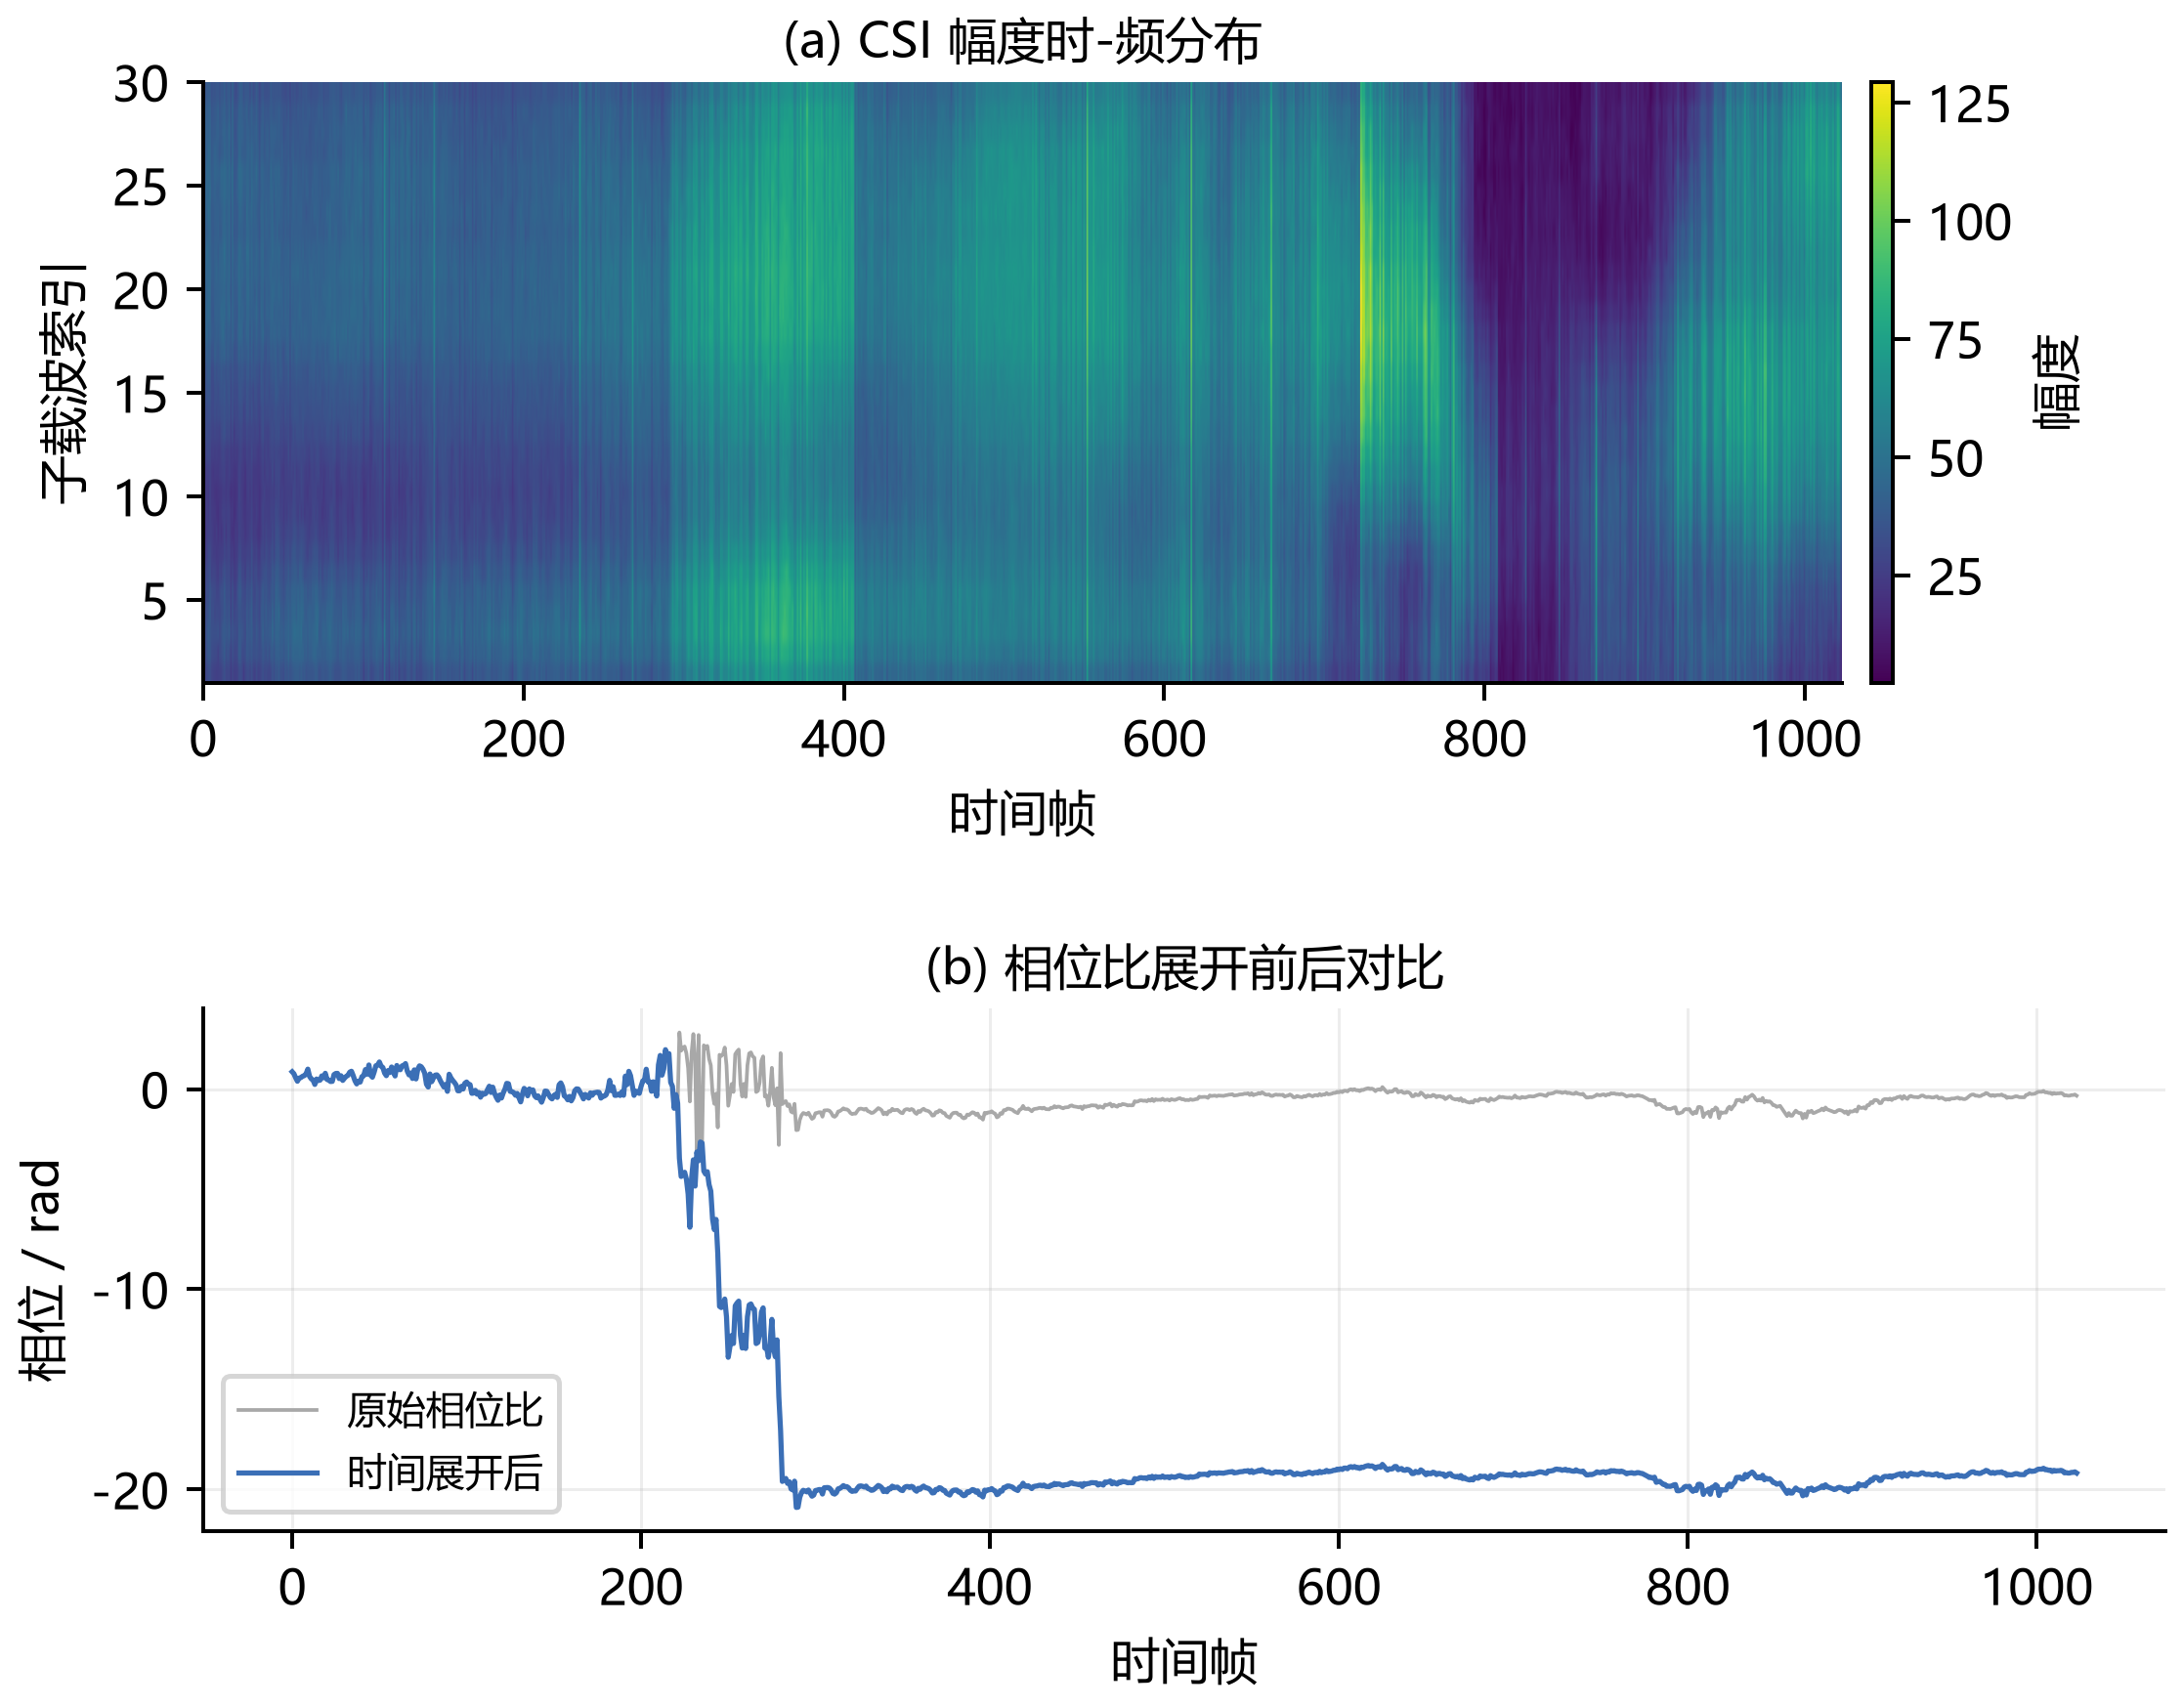
\includegraphics[width=0.92\textwidth]{figures/csi_signal_example.png}
\caption{真实 CSI 样例及接收天线相位比的时间展开效果}
\label{fig:csi_signal_example}
\end{figure}

\section{滑动窗口组织}
原始 CSI 文件通常包含连续采集得到的一整段时间序列，不同文件的长度可能存在差异。为了统一处理长序列，本文采用长度为 512、步长为 256 的滑动窗口切分相位比序列。设窗口长度为 $L$、滑动步长为 $P$，则第 $k$ 个窗口可表示为
\begin{equation}
W_k=\left[\tilde{\theta}_{kP},\tilde{\theta}_{kP+1},\ldots,\tilde{\theta}_{kP+L-1}\right].
\end{equation}

窗口化的作用是将长 CSI 文件分解为若干局部时间片段，使后续特征统计能够同时覆盖局部变化和整段采集过程。本文最终分类单位仍为完整原始文件，而不是单个窗口。这样能够避免仅凭短时间片段判断整体脊柱姿态，同时保留同一文件内多个窗口所包含的时间变化信息。

窗口长度决定单个局部片段覆盖的时间范围。窗口过短时，统计量容易受到瞬时噪声影响，难以反映相对稳定状态；窗口过长时，局部变化可能被过度平滑，并增加不同长度序列之间的处理差异。滑动步长则决定相邻窗口的重叠程度：较小步长可以提高时间覆盖的连续性，但会产生更多高度相关的窗口。因此，窗口参数应综合考虑信号持续时间、局部稳定性和计算开销，并且必须在验证集上选择，不能根据测试集结果反向调整。

对于长度不足一个完整窗口的序列，可以采用丢弃、补齐或变长统计等处理方式。不同策略会改变有效样本信息，因此应在训练和检测阶段保持一致，并记录短序列处理规则。对于长序列，窗口化只用于组织特征计算，同一原始文件产生的窗口始终属于同一数据子集，避免重叠片段跨越训练集与测试集。

\section{文件级统计特征}
在完成窗口化后，系统将同一原始文件产生的全部窗口重新聚合，并对每个相位比特征计算统计量。当前每一时间帧整理得到 180 个相位比特征；对每个特征计算 9 组统计量，包括均值、标准差、10\% 分位数、中位数、90\% 分位数、相邻帧差分绝对值均值、相邻帧差分标准差、相位正弦均值和相位余弦均值。因此，每个原始文件最终形成
\begin{equation}
180\times 9=1620
\end{equation}
维文件级特征向量。

这些统计量分别描述相位比序列的整体水平、波动程度、分布位置、动态变化和周期性信息。分位数统计可降低少量异常帧对特征的影响；差分统计刻画姿态相关扰动在时间上的变化强度；正弦和余弦统计保留相位特征的周期性质。通过文件级聚合，系统将连续 CSI 信号转化为固定长度向量，为 ExtraTrees 分类器提供稳定输入。

从特征含义看，均值和分位数主要描述序列的位置与分布范围，标准差描述整体离散程度，差分特征描述相邻时刻变化强度。由于相位属于周期变量，直接对展开后的数值求均值可能受到累计周期变化影响，正弦均值和余弦均值则可以从圆周统计角度表达相位集中方向。多类统计量共同使用，使固定长度向量同时包含分布、动态和周期信息。

\section{特征处理的稳定性原则}
为了保证分类结果能够被正确解释，特征处理流程需要满足一致性、稳健性和隔离性三个原则。一致性要求训练、验证和检测阶段采用完全相同的天线顺序、子载波顺序、窗口规则和统计量定义；稳健性要求对分母接近零、非有限数值、异常跳变和长度不足等情况进行统一处理；隔离性要求所有依赖数据分布的处理参数仅从训练集获得，测试集不得参与阈值选择或特征筛选。

此外，固定长度表示虽然便于传统分类器处理，但会压缩原始时间顺序信息。统计聚合适合描述相对稳定姿态的总体规律，却可能无法完整表达快速、短暂或顺序相关的动作过程。因此，特征表示必须与研究对象匹配：对于稳定状态，可以强调分布和变化强度；对于复杂动作，则可能需要保留更完整的时序结构。

\section{本章小结}
本章建立了从多维复数 CSI 到文件级统计表示的处理过程。首先分析人体姿态通过多径传播影响信道响应的基本机理，并说明原始相位中的公共偏移和链路误差；随后利用接收天线复数比值构造相对相位，通过时间展开和滑动窗口组织连续序列；最后使用分布、差分和周期统计量形成固定长度特征。上述步骤的核心目标是在保留姿态相关差异的同时，提高不同处理阶段的数据一致性和表示稳定性。

% !TEX TS-program = XeLaTeX
% !TEX encoding = UTF-8 Unicode

\chapter{基于相位比统计特征的脊柱姿态检测方法}
\label{chap03}
\defaultfont

\section{问题定义}
本文将脊柱姿态检测建模为基于 WiFi CSI 的文件级三分类问题。设一个原始 CSI 文件为 $X$，其对应的姿态标签集合为
\begin{equation}
\mathcal{Y}=\{y_1,y_2,y_3\},
\end{equation}
其中 $y_1$、$y_2$ 和 $y_3$ 分别表示正常姿态、脊柱后凸相关姿态和脊柱侧弯相关姿态。模型的目标是从 CSI 文件中提取能够反映人体姿态差异的特征，并学习特征向量到姿态类别之间的映射关系：
\begin{equation}
\hat{y}=f(X), \quad \hat{y}\in \mathcal{Y}.
\end{equation}

在无线感知场景中，人体位于发射端与接收端之间时，会对无线信号产生反射、遮挡、散射和多径传播等影响。不同脊柱姿态会改变人体躯干形态及其对无线传播路径的扰动方式，从而使 CSI 的相位比序列呈现出可区分的统计特征。本文利用这一特性进行非接触式脊柱姿态检测。

该问题建立在三个基本假设之上：采集阶段的类别标签能够反映预先定义的姿态状态；待检测数据与训练数据具有一致的 CSI 维度和链路排列；单个原始文件在其采集时段内主要对应一种姿态。若输入数据不满足这些条件，例如同时包含多种姿态转换或缺少必要天线链路，则固定长度文件级分类结果的含义需要重新评估。

\section{方法总体框架}
本文方法由 CSI 数据解析、接收天线相位比计算、相位展开、滑动窗口组织、文件级统计特征聚合、ExtraTrees 分类和检测结果输出组成。整体流程可表示为
\begin{equation}
X_{\mathrm{raw}}
\rightarrow X_{\mathrm{csi}}
\rightarrow X_{\mathrm{ratio}}
\rightarrow X_{\mathrm{stat}}
\rightarrow g(X_{\mathrm{stat}})
\rightarrow \hat{y},
\end{equation}
其中 $X_{\mathrm{raw}}$ 表示原始采集文件，$X_{\mathrm{csi}}$ 表示解析后的复数 CSI 数据，$X_{\mathrm{ratio}}$ 表示相位比序列，$X_{\mathrm{stat}}$ 表示文件级统计特征，$g(\cdot)$ 表示 ExtraTrees 分类器，$\hat{y}$ 表示最终输出的脊柱姿态类别。

系统首先从原始 \texttt{.dat} 文件中解析复数 CSI，获得时间帧、子载波、接收天线和发射天线维度上的信道响应；然后以第 0 根接收天线为参考，计算其他接收天线与参考天线之间的复数比值，并取幅角得到相位比；随后沿时间维度进行相位展开，减少相位周期跳变带来的不连续；最后将整个文件聚合为 1620 维统计特征，并输入 ExtraTrees 分类器进行三分类预测。

\section{文件级特征构建}
本文不直接将单个窗口作为最终分类对象，而是将一个原始 CSI 文件作为一次检测样本。这样做的原因是，脊柱姿态属于相对稳定的身体状态，单个短窗口可能只包含局部扰动，而完整文件能够更充分地保留一段采集过程中的整体统计规律。

对每个原始文件，系统首先生成长度为 512、步长为 256 的滑动窗口。每个窗口继承其所属文件的姿态标签，但窗口仅用于组织和统计特征，不作为最终投票单位。随后，系统汇总该文件全部窗口中的相位比序列，并对每一维相位比特征计算以下统计量：
\begin{enumerate}
\item 均值，用于描述相位比的整体水平；
\item 标准差，用于描述相位比的波动程度；
\item 10\% 分位数、中位数和 90\% 分位数，用于描述相位比分布；
\item 相邻帧差分绝对值均值，用于描述时间变化强度；
\item 相邻帧差分标准差，用于描述变化过程的稳定性；
\item 相位正弦均值和余弦均值，用于保留相位的周期性信息。
\end{enumerate}

由于每一时间帧具有 180 个相位比特征，每个特征对应 9 个统计量，因此每个 CSI 文件被表示为 1620 维文件级特征向量。该向量既包含整段采集数据的总体分布，也包含局部时间变化信息，能够作为传统机器学习分类器的输入。

\section{文件级建模与数据隔离}
本文选择文件级建模的另一个重要原因是控制数据相关性。采用重叠滑动窗口时，相邻窗口共享大量时间帧。如果将窗口随机划分到训练集、验证集和测试集，同一原始序列中的近似片段可能出现在不同子集中，使模型间接接触测试信息。即使最终指标较高，也难以判断模型学习到的是姿态规律还是原始序列的局部特征。

因此，完整流程应首先以原始文件或更高层级的独立采集单元划分数据，再分别执行窗口化和统计聚合。训练集用于学习模型参数，验证集用于比较模型和选择配置，测试集只用于最终评价。若研究目标是评价对陌生人员的泛化能力，还应进一步以受试者为分组单位进行划分，保证同一受试者的数据不会跨越训练集和测试集。

\section{ExtraTrees 分类模型}
ExtraTrees 即极端随机树集成模型，是一种由多棵随机决策树组成的监督分类方法。与普通决策树相比，ExtraTrees 在训练每棵树时引入更强的随机性：模型不仅随机选择候选特征，还随机生成候选切分阈值，再从中选择划分效果较好的节点切分方式。多棵树分别给出分类结果后，集成模型通过投票或概率平均输出最终类别。

设文件级统计特征为 $x\in \mathbb{R}^{1620}$，第 $m$ 棵树的预测结果为 $h_m(x)$，则由 $M$ 棵树组成的 ExtraTrees 分类器可表示为
\begin{equation}
g(x)=\operatorname{mode}\{h_1(x),h_2(x),\ldots,h_M(x)\}.
\end{equation}
本文最终模型使用 $M=700$ 棵极端随机树，并采用类别平衡权重、平方根特征采样和固定随机种子。类别平衡权重用于减小类别样本数量差异带来的影响；平方根特征采样使每棵树在不同特征子空间上学习分类规则；固定随机种子保证实验结果可复现。

ExtraTrees 适合本文任务的主要原因在于：首先，当前数据集文件数量有限，而统计特征维度较高，树集成模型能够在小样本高维特征上获得稳定表现；其次，树模型不依赖严格的特征缩放，对不同量纲的统计特征具有较好兼容性；最后，多棵树的集成能够表达复杂的非线性特征组合，适合处理多天线、多子载波 CSI 特征之间的交互关系。

\section{训练与分类决策机制}
模型训练阶段仅使用训练集中的文件级特征估计树节点的划分规则。验证集用于比较候选模型、树数量、特征采样方式和类别权重等配置。模型配置确定后，测试集保持封闭，直至最终性能评价。该顺序能够减少反复查看测试结果造成的选择偏差，使测试指标更接近一次独立评价。

对于单个待检测文件，每棵树根据其学习到的节点规则给出类别判断，集成模型再通过投票或类别概率平均形成最终结果。如果应用场景需要表达不确定性，可以同时保留各类别的投票比例或预测概率，并设置低置信度拒绝机制。拒绝机制不改变分类模型本身，而是在证据不足时避免输出过于确定的类别。由于本文实验主要评价三分类性能，最终结果仍以离散类别和分类指标为主。

为分析最终模型实际使用的信息，本文进一步统计 700 棵树基于不纯度下降得到的特征重要性，并分别按统计量类型聚合及列出重要性最高的具体特征，如图~\ref{fig:extratrees_importance} 所示。正弦均值与余弦均值的累计贡献最高，二者合计约占总重要性的 40\%，说明保留相位周期结构对分类具有明显作用；差分绝对值均值与差分标准差也占有较高权重，表明时间变化强度是姿态区分的重要依据。排名靠前的具体特征主要集中在若干子载波的 RX2/RX1 相位比链路。需要指出的是，该重要性反映模型内部的相对分裂贡献，不表示特征与姿态之间存在直接因果关系。

\begin{figure}[htbp]
\centering
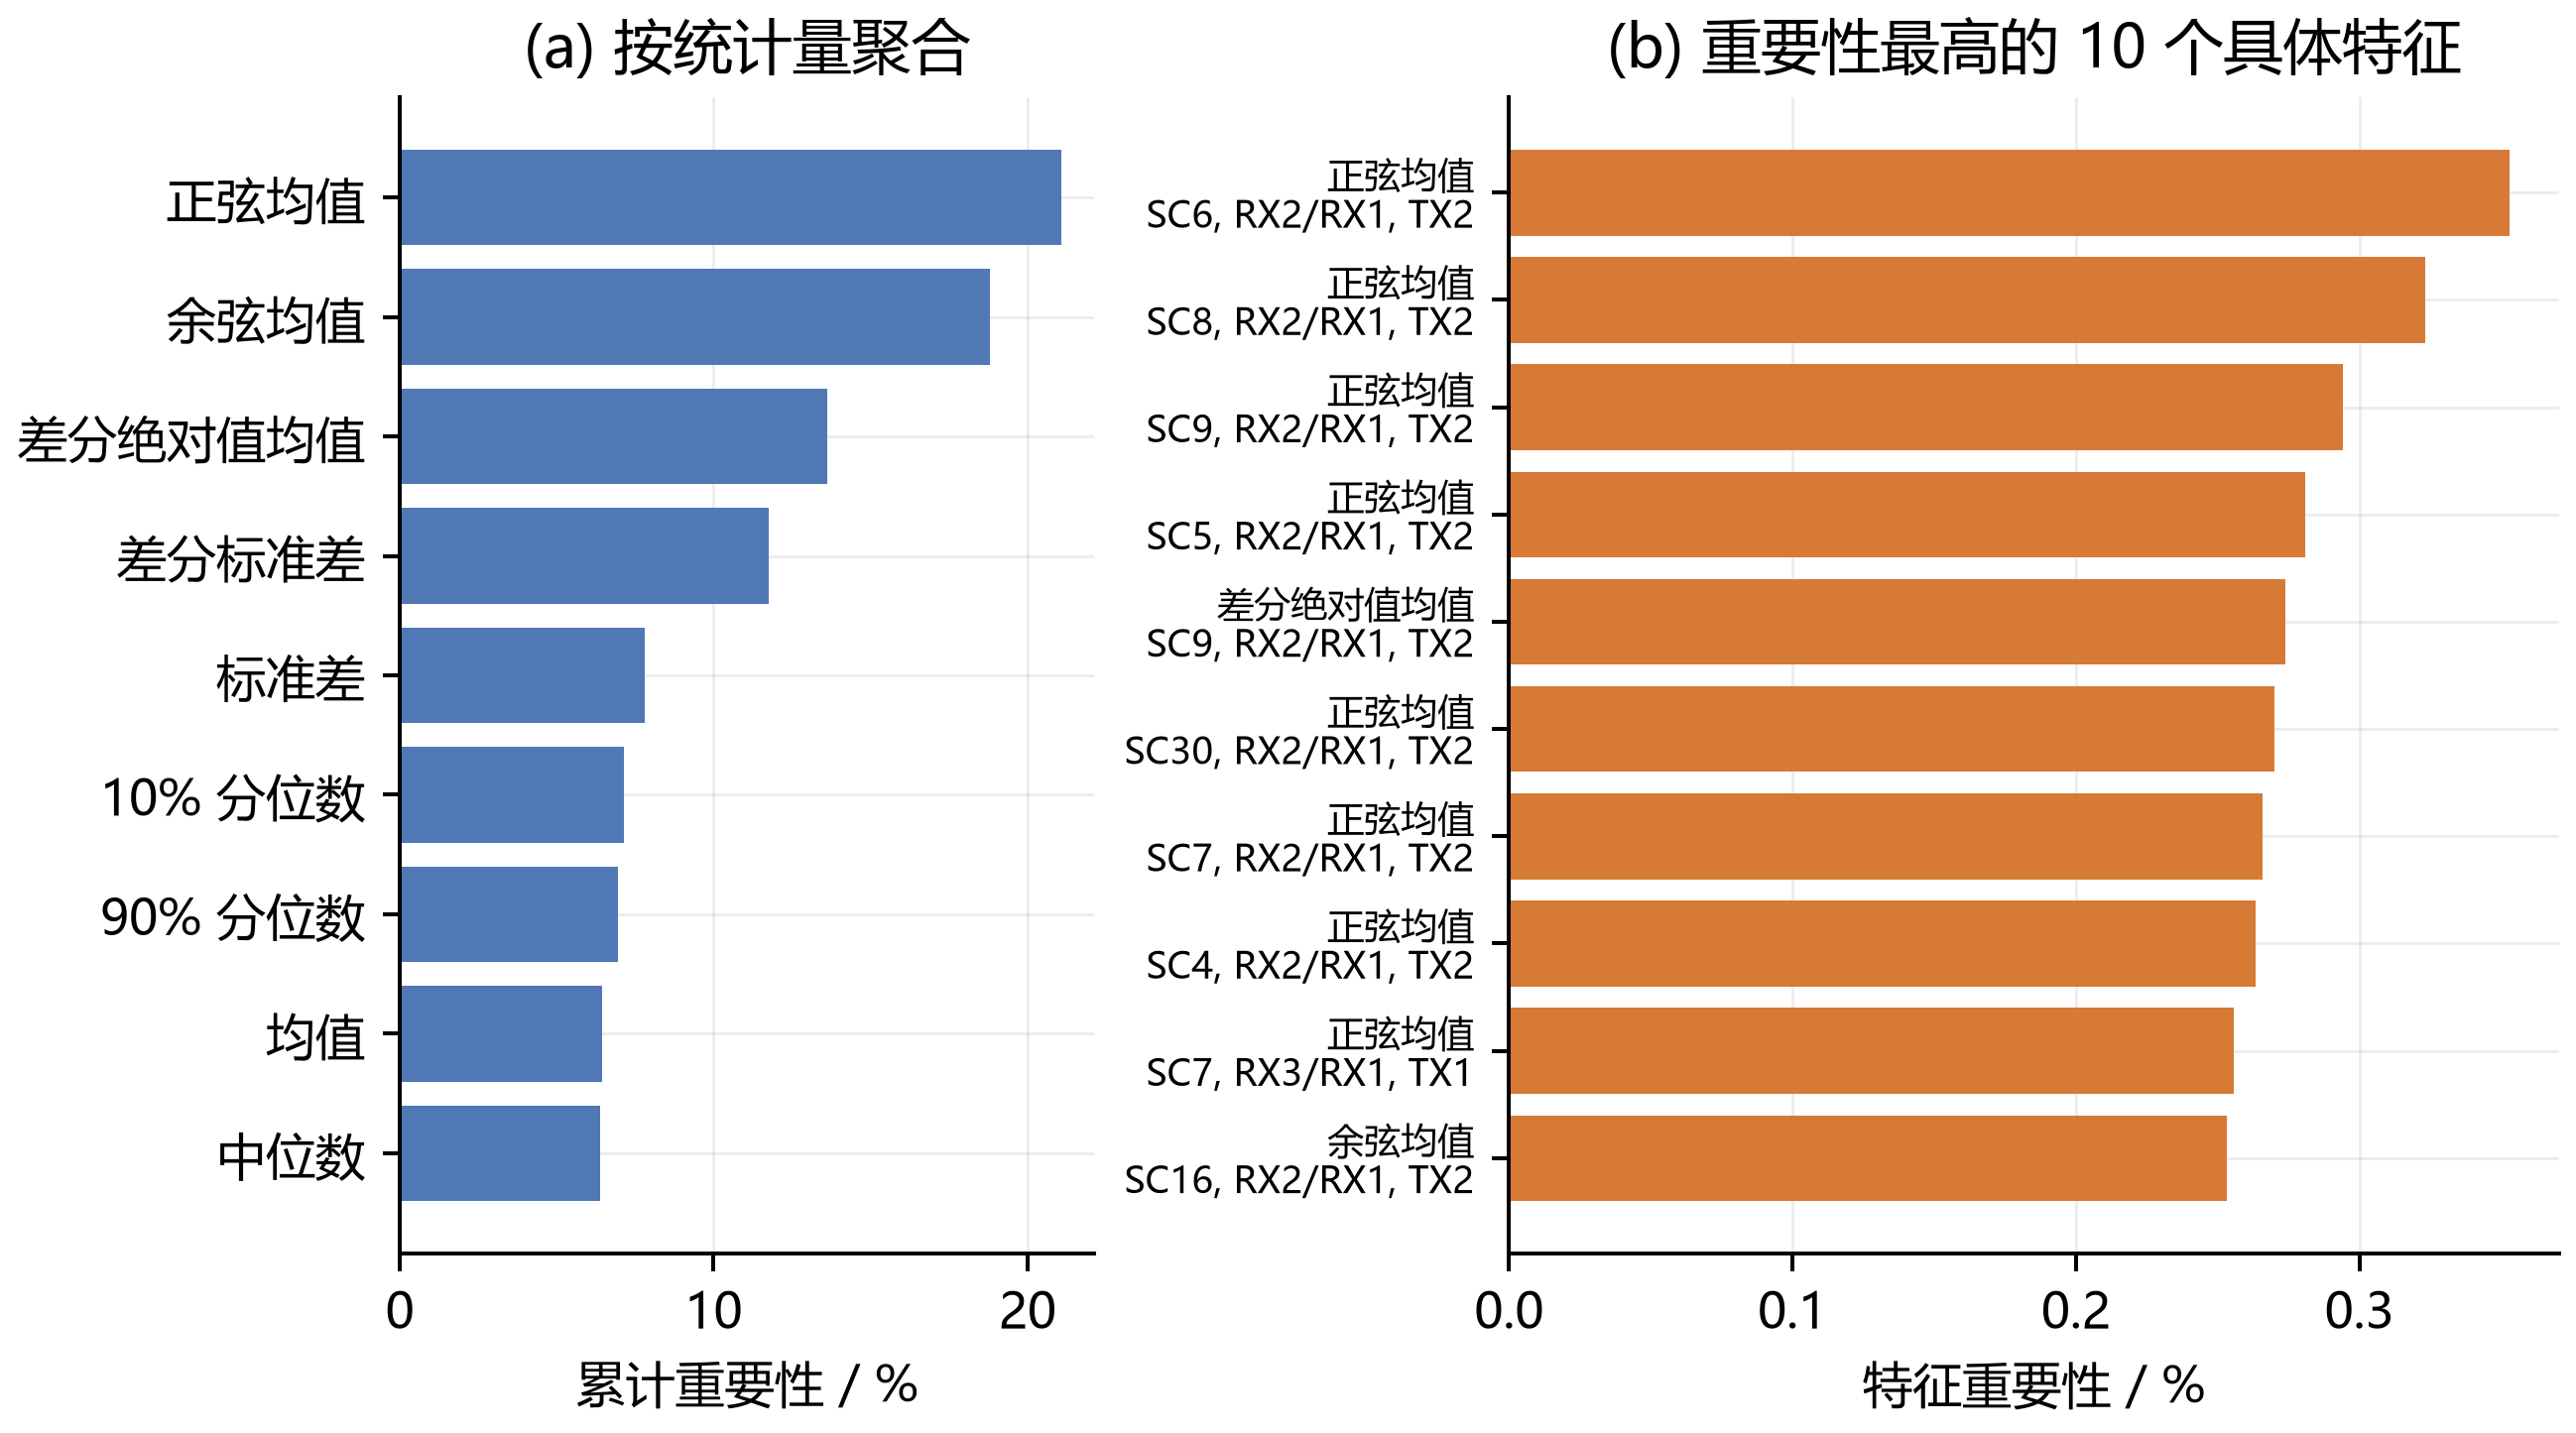
\includegraphics[width=0.96\textwidth]{figures/extratrees_feature_importance.png}
\caption{ExtraTrees 模型的特征重要性分析}
\label{fig:extratrees_importance}
\end{figure}

\section{检测结果输出}
检测阶段对待检测 CSI 文件执行与训练阶段相同的数据处理流程。系统解析复数 CSI，计算接收天线相位比并进行时间相位展开，随后生成滑动窗口并聚合为 1620 维文件级统计特征。训练完成的 ExtraTrees 模型根据该特征向量输出三类姿态的预测结果。

该流程实现了从 WiFi CSI 原始文件到脊柱姿态类别的完整检测。由于检测过程不依赖摄像头图像或可穿戴设备，系统具有非接触、低侵入和隐私友好的特点，适用于室内场景下的人体姿态感知与脊柱健康辅助检测研究。

\section{算法流程与复杂度分析}
从算法结构看，方法可以概括为数据解析、相对相位构造、时间组织、统计聚合和集成分类五个阶段。训练阶段在上述特征处理之后增加模型拟合和配置选择，检测阶段则加载已经确定的模型执行分类。两个阶段共享同一特征构建过程，从而避免训练与检测使用不同处理规则。

设单个文件包含 $T$ 个时间帧，每帧相位比维度为 $D$，统计量数量为 $K$。相位比计算、时间展开和统计聚合的主要计算量随 $T$ 和 $D$ 近似线性增长，生成的文件级向量维度为 $D K$。对于包含 $M$ 棵树的集成模型，单次分类需要沿每棵树的决策路径进行判断，其开销与树数量和平均树深相关。与直接对长序列执行多层神经网络相比，文件级统计表示能够在分类阶段降低输入规模，但代价是压缩部分精细时序信息。

该复杂度分析说明，方法适合以完整采集文件为单位进行批量训练和检测。若扩展到实时连续监测，需要进一步设计增量窗口更新、在线质量检查和连续结果平滑机制，而不能简单地将离线文件分类结果等同于实时输出。

\section{本章小结}
本章将脊柱姿态检测形式化为文件级监督分类问题，并给出了从原始 CSI 到类别输出的完整方法。通过先划分原始文件、再生成窗口，可以降低高度相关片段跨越数据子集造成的信息泄漏风险；通过文件级统计表示和 ExtraTrees 集成决策，可以在有限样本和高维特征条件下建立分类模型。最后，本章讨论了训练与检测的一致性、低置信度输出以及方法的计算复杂度，为后续实验设计提供依据。

% !TEX TS-program = XeLaTeX
% !TEX encoding = UTF-8 Unicode

\chapter{实验设计与结果分析}
\label{chap:experiment}
\defaultfont

\section{实验目标}
实验部分围绕基于 WiFi CSI 的脊柱姿态检测方法展开，验证接收天线相位比、文件级统计特征和 ExtraTrees 分类器在三类姿态识别任务中的有效性。实验目标包括：检验 CSI 相位比特征是否能够反映不同脊柱姿态差异；比较 TCN、SVM、Random Forest 和 ExtraTrees 等模型的分类效果；分析最终模型在测试集上的准确率、精确率、召回率、F1 值和混淆矩阵表现。

\section{研究问题}
为了使实验过程与研究目标相对应，本文将评价内容归纳为三个研究问题。第一个问题是，在统一的数据划分条件下，基于文件级统计特征的传统分类模型能否获得稳定的三分类结果；第二个问题是，ExtraTrees 与其他候选模型相比是否具有更好的留出测试表现；第三个问题是，不同类别的错误分布是否存在明显差异，以及这些差异能够说明哪些方法局限。

上述问题分别对应方法可行性、模型选择和错误解释三个层面。实验结果只能在给定受试者和相近采集条件下回答这些问题，不能直接证明模型已经具备跨人员、跨环境或临床应用能力。对实验结论的适用范围进行限定，是保证评价结果不被过度解释的重要前提。

\section{数据集与划分方式}
实验数据集共包含 750 个 CSI 原始文件，类别包括 \texttt{kyphosis}、\texttt{normal} 和 \texttt{scoliosis}，分别对应脊柱后凸相关姿态、正常姿态和脊柱侧弯相关姿态。三类样本数量均为 250 个，数据来自 5 位受试者。

图~\ref{fig:dataset_composition} 按受试者与姿态类别展示了原始文件构成。每位受试者在三种姿态下均采集 50 个文件，因而类别与受试者维度均保持平衡，可减少由样本数量差异造成的评价偏差。

\begin{figure}[htbp]
\centering
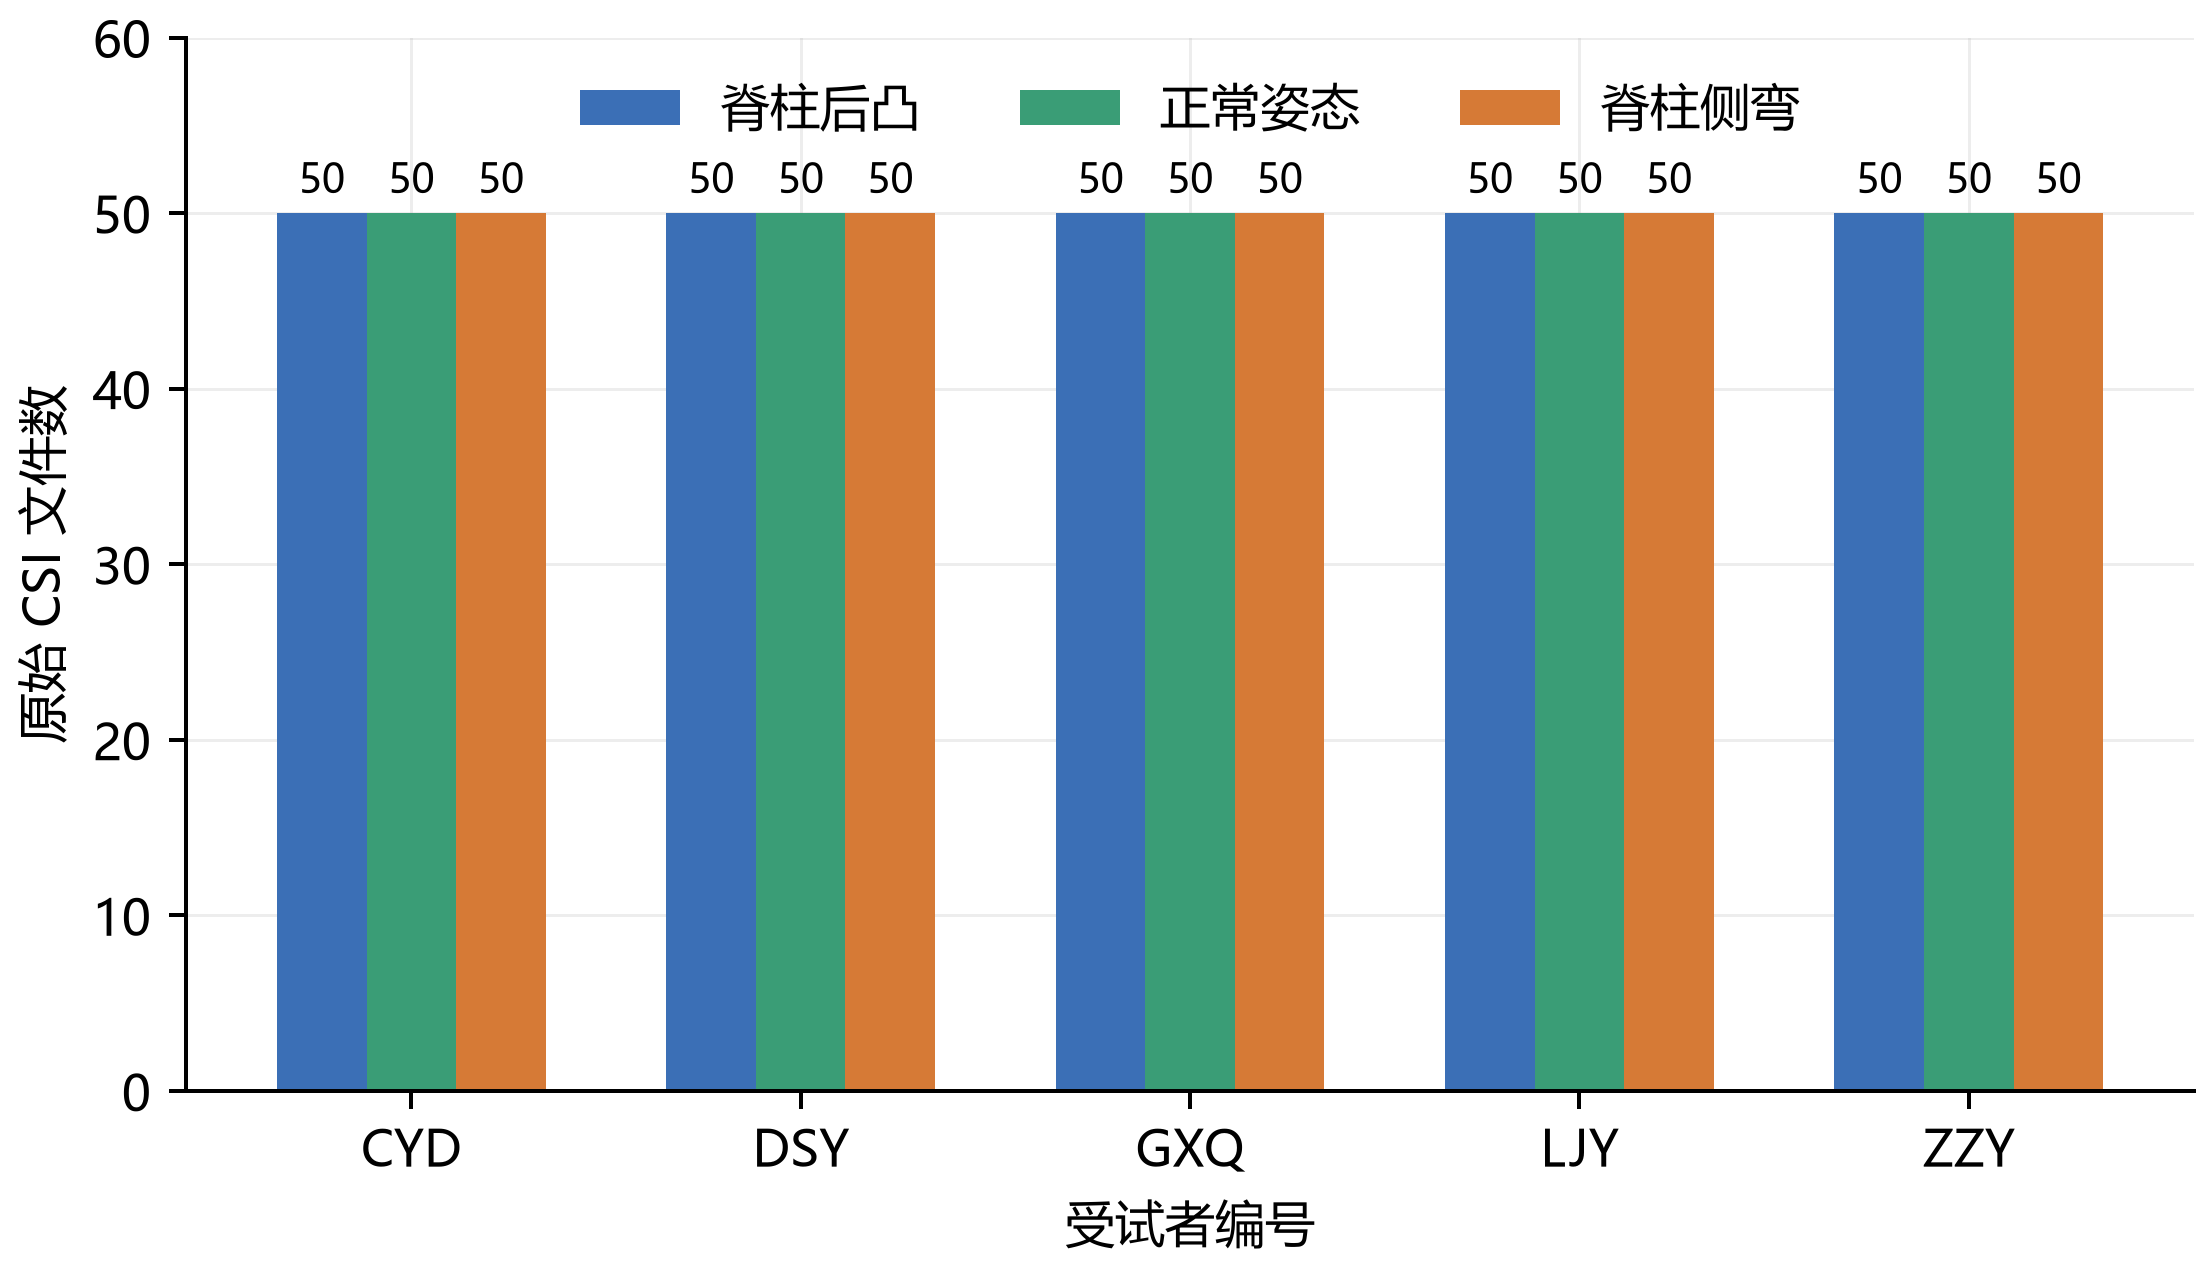
\includegraphics[width=0.88\textwidth]{figures/dataset_composition.png}
\caption{不同受试者与姿态类别的 CSI 文件数量}
\label{fig:dataset_composition}
\end{figure}

数据集采用固定随机种子 42 在原始文件级别进行划分。训练集包含 524 个文件，占 69.9\%；验证集包含 113 个文件，占 15.1\%；测试集包含 113 个文件，占 15.1\%。划分发生在滑动窗口生成之前，因此同一原始文件产生的重叠窗口不会同时出现在训练集和测试集中。

\begin{table}[htbp]
\centering
\song\wuhao
\caption{数据集划分情况}
\label{tab:dataset_split}
\begin{tabular}{cccc}
\hline
数据集 & 文件数 & 比例 & 用途 \\
\hline
训练集 & 524 & 69.9\% & 模型参数学习 \\
验证集 & 113 & 15.1\% & 模型选择与配置比较 \\
测试集 & 113 & 15.1\% & 最终性能评估 \\
\hline
\end{tabular}
\end{table}

各子集内部的类别数量如图~\ref{fig:dataset_split} 所示。训练、验证和测试子集均近似保持三类均衡，其中测试集三类文件数分别为 37、38 和 38。

\begin{figure}[htbp]
\centering
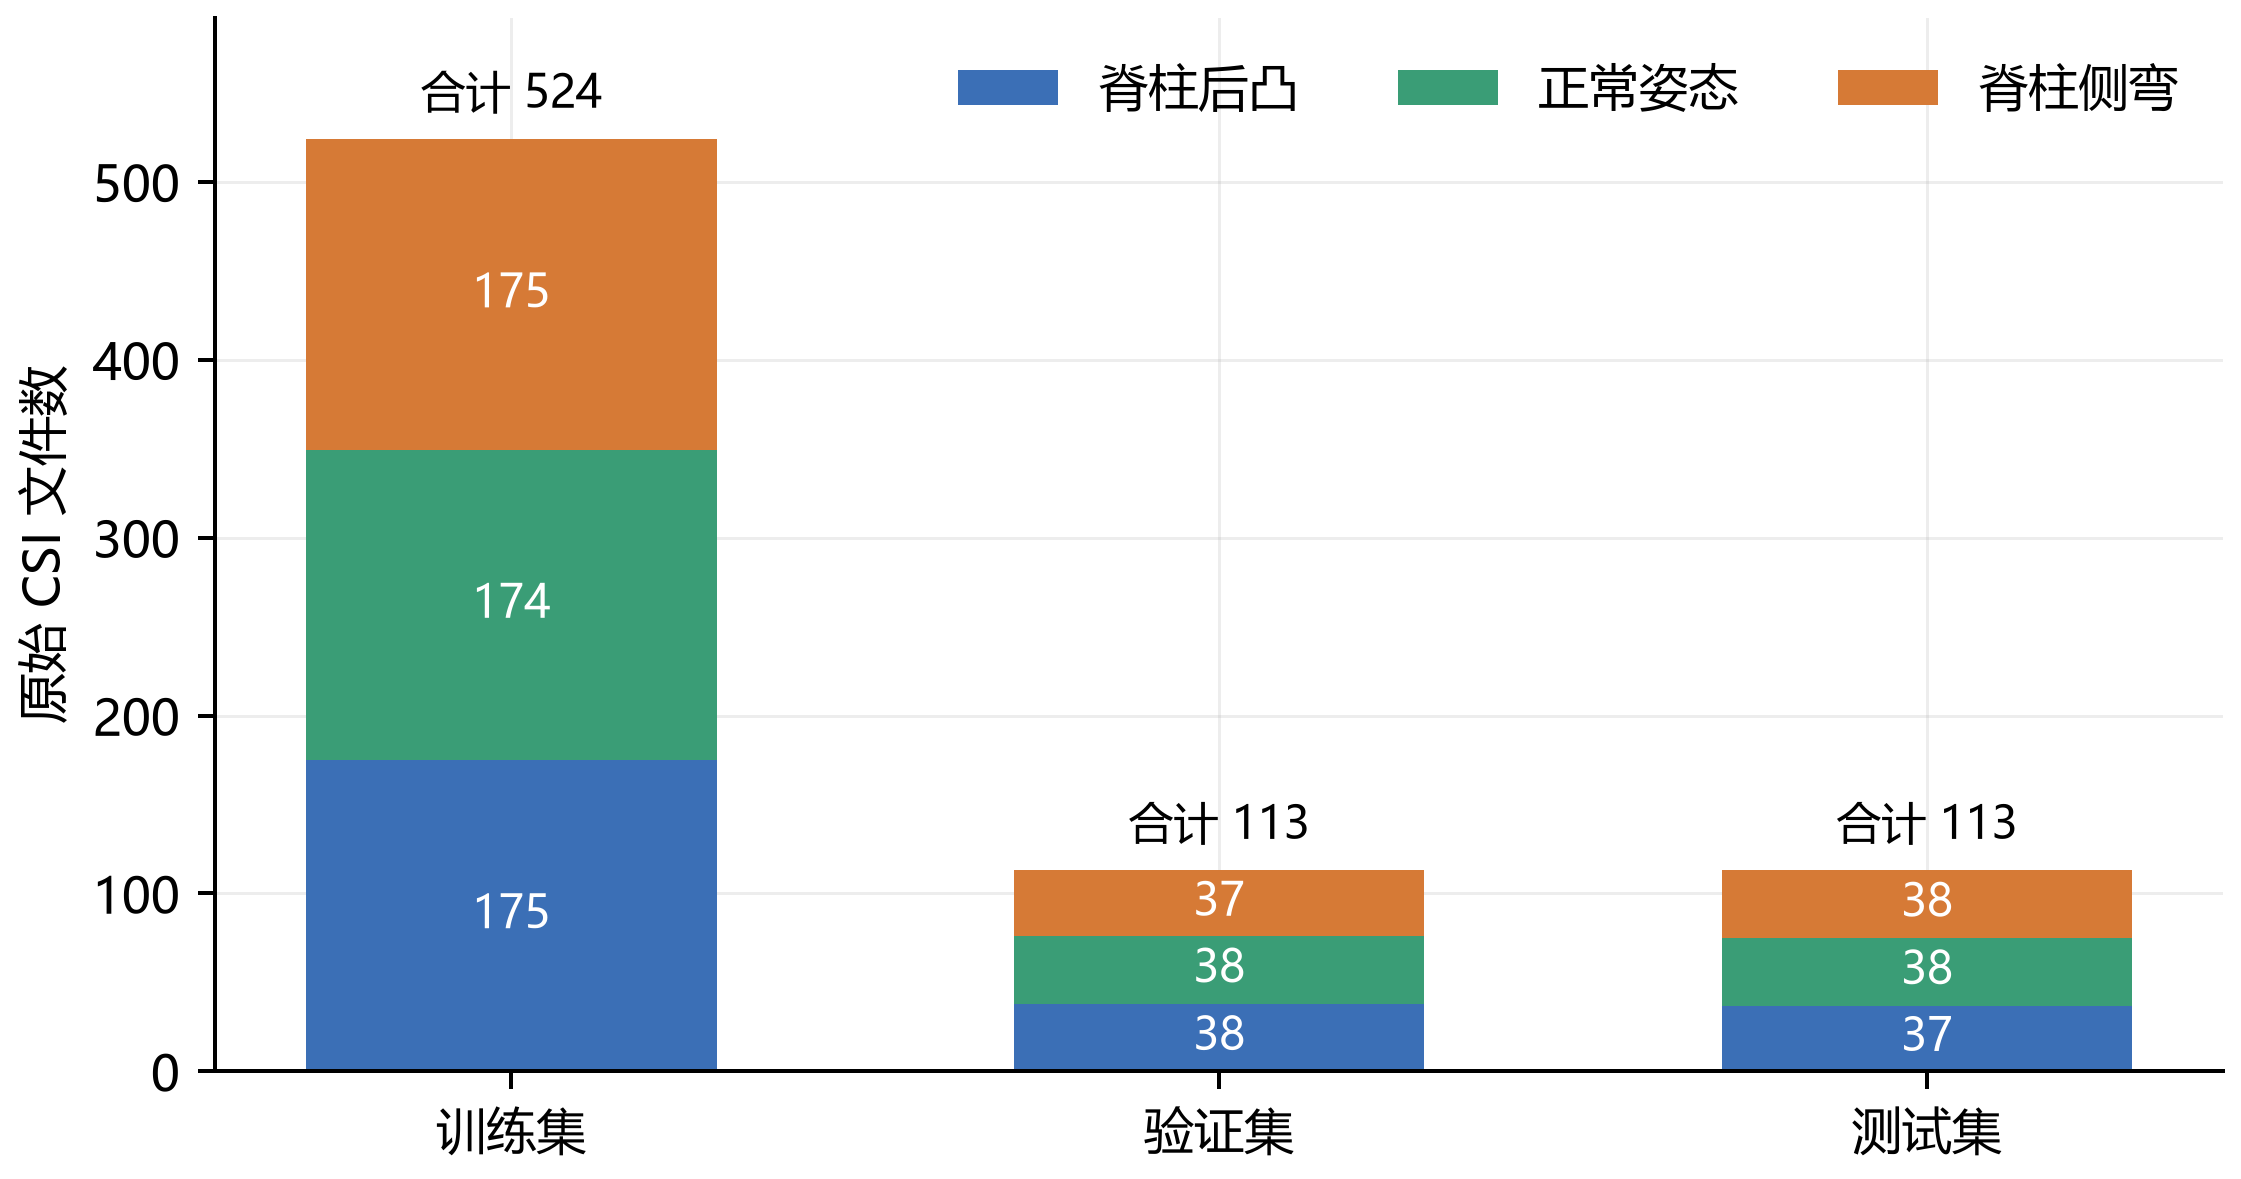
\includegraphics[width=0.82\textwidth]{figures/dataset_split.png}
\caption{训练集、验证集与测试集的类别分布}
\label{fig:dataset_split}
\end{figure}

\section{实验协议与信息隔离}
实验协议按照训练、验证和测试三个阶段组织。训练集用于学习分类模型的参数；验证集用于比较候选模型及其配置；测试集在模型方案确定前保持隔离，仅用于报告最终性能。所有滑动窗口和文件级特征均在原始文件划分完成后生成，避免同一文件产生的重叠窗口进入不同数据子集。

对于 TCN 与传统分类模型的比较，需要注意两类方法的输入单位不同。TCN 使用局部时间窗口，文件级模型使用完整采集文件的统计表示，因此对比结果反映的是“表示方式与分类器组合”的整体差异，而不能仅归因于分类器结构。本文保留该对比用于说明不同建模路线在当前数据条件下的实际表现，同时在结果解释中避免把差异简单表述为某一类模型在所有 CSI 任务中普遍更优。

实验过程中还应保持标签映射、特征维度、随机种子和评价脚本一致。模型配置只能依据训练集与验证集确定，测试集上的分类报告、混淆矩阵和汇总指标由同一组预测结果计算。通过保存数据划分和模型配置，可以在独立运行时重新生成评价结果，并检查训练阶段与检测阶段是否采用一致的数据处理流程。

\section{评价指标}
为了全面评价模型分类效果，实验采用准确率、精确率、召回率和 F1 值作为主要指标。准确率表示预测正确的样本占总样本的比例：
\begin{equation}
Accuracy=\frac{TP+TN}{TP+TN+FP+FN}.
\end{equation}

精确率表示被预测为某一类别的样本中真实属于该类别的比例：
\begin{equation}
Precision=\frac{TP}{TP+FP}.
\end{equation}

召回率表示真实属于某一类别的样本中被正确识别的比例：
\begin{equation}
Recall=\frac{TP}{TP+FN}.
\end{equation}

F1 值综合衡量精确率和召回率：
\begin{equation}
F1=\frac{2\times Precision\times Recall}{Precision+Recall}.
\end{equation}

此外，实验使用混淆矩阵分析不同姿态类别之间的误分情况。混淆矩阵能够直观展示每个真实类别被预测为各类别的数量，有助于观察模型在哪些类别之间更容易混淆。

对于多分类任务，精确率、召回率和 F1 值可以分别按类别计算，再采用宏平均或加权平均形成总体指标。宏平均对每个类别赋予相同权重，适合观察类别均衡条件下的整体表现；加权平均则按照各类别样本数量加权。本文数据集类别数量近似均衡，因此准确率与宏平均指标可以相互补充，但仍需结合逐类结果和混淆矩阵分析，避免单一汇总数值掩盖特定类别的系统性错误。

\section{模型配置选择原则}
候选模型的配置选择遵循“训练集拟合、验证集选择、测试集确认”的原则。对于支持向量机，需要关注核函数、正则化强度和核参数；对于树集成模型，需要关注树数量、候选特征数量、类别权重和叶节点约束；对于时序神经网络，还需要考虑网络深度、感受野、优化过程和早停策略。不同模型的参数含义不同，不宜通过比较参数数量判断其复杂程度。

验证集性能最高并不必然意味着模型具有最好的测试泛化能力。当多个配置的验证结果接近时，应优先考虑结果稳定、结构较简单且计算开销可控的方案。测试集只用于在方案确定后进行一次独立确认，不应根据测试结果继续修改特征或模型，否则测试集会逐渐承担验证集的作用，导致最终性能估计偏乐观。

\section{模型对比实验}
为确定最终分类模型，本文比较了 TCN、RBF SVM、Random Forest 和 ExtraTrees 四种方案。TCN 为早期窗口级深度学习基线，输入为 512 帧 CSI 窗口；SVM、Random Forest 和 ExtraTrees 均使用文件级相位比统计特征。模型对比结果如表 4.2 所示。

\begin{table}[htbp]
\centering
\song\wuhao
\caption{不同模型实验结果对比}
\label{tab:model_compare}
\begin{tabular}{ccccc}
\hline
模型 & 输入单位 & 验证准确率 & 测试准确率 & 测试宏平均 F1 \\
\hline
TCN & 512 帧窗口 & 56.12\% & 50.30\% & 50.16\% \\
RBF SVM & 文件统计特征 & 约 92.04\% & 约 89.38\% & -- \\
Random Forest & 文件统计特征 & 约 96.46\% & 约 90.27\% & -- \\
ExtraTrees & 文件统计特征 & 95.58\% & 92.04\% & 92.08\% \\
\hline
\end{tabular}
\end{table}

图~\ref{fig:model_comparison} 对表~\ref{tab:model_compare} 中的验证和测试准确率作了直观比较。采用文件级统计特征的三种传统模型均明显优于窗口级 TCN；ExtraTrees 的验证结果略低于 Random Forest，但取得最高的测试准确率，显示出更好的留出集泛化表现。

\begin{figure}[htbp]
\centering
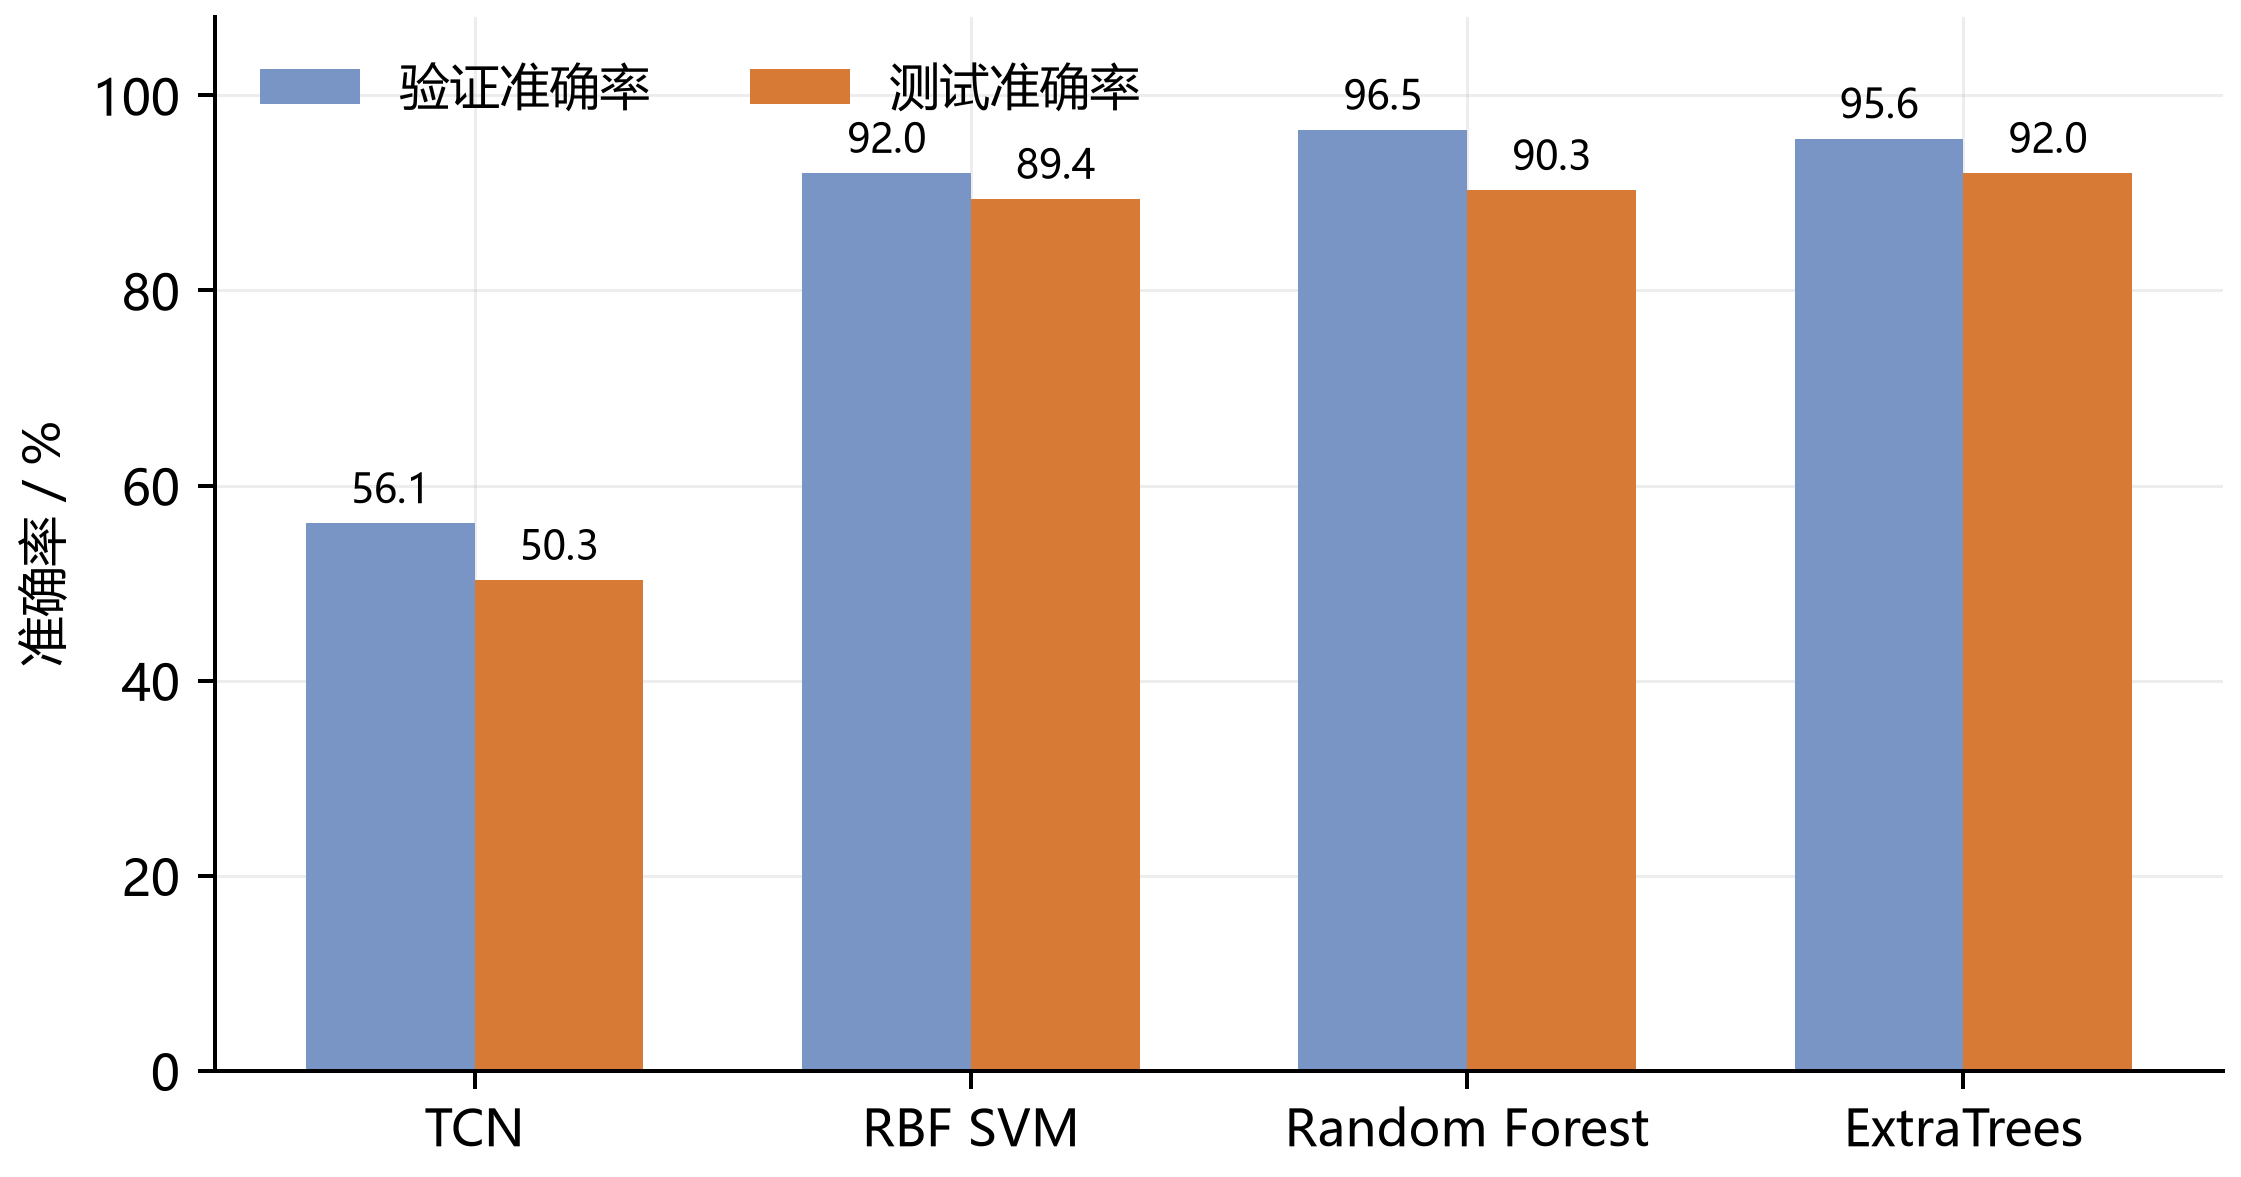
\includegraphics[width=0.88\textwidth]{figures/model_comparison.png}
\caption{不同分类模型的验证集与测试集准确率对比}
\label{fig:model_comparison}
\end{figure}

从实验结果可以看出，TCN 在当前数据规模下测试表现较低，说明仅使用窗口级深度模型难以稳定学习到可泛化的姿态差异。RBF SVM 和 Random Forest 在文件级统计特征上表现明显提升，其中 Random Forest 测试准确率已达到 90.27\%。ExtraTrees 进一步取得 92.04\% 的测试准确率和 92.08\% 的宏平均 F1 值，因此本文选用 ExtraTrees 作为最终分类模型。

\section{最终测试结果}
最终 ExtraTrees 模型在 113 个测试文件上正确分类 104 个文件，测试准确率为 92.04\%。各类别的精确率、召回率和 F1 值如表 4.3 所示。

\begin{table}[htbp]
\centering
\song\wuhao
\caption{ExtraTrees 模型测试集分类结果}
\label{tab:final_result}
\begin{tabular}{ccccc}
\hline
类别 & Precision & Recall & F1 & 正确数/总数 \\
\hline
\texttt{kyphosis} & 87.18\% & 91.89\% & 89.47\% & 34/37 \\
\texttt{normal} & 90.00\% & 94.74\% & 92.31\% & 36/38 \\
\texttt{scoliosis} & 100.00\% & 89.47\% & 94.44\% & 34/38 \\
宏平均 & 92.39\% & 92.03\% & 92.08\% & 104/113 \\
\hline
\end{tabular}
\end{table}

混淆矩阵的类别顺序为 \texttt{kyphosis}、\texttt{normal}、\texttt{scoliosis}，结果为
\begin{equation}
\begin{bmatrix}
34 & 3 & 0 \\
2 & 36 & 0 \\
3 & 1 & 34
\end{bmatrix}.
\end{equation}

\begin{figure}[htbp]
\centering
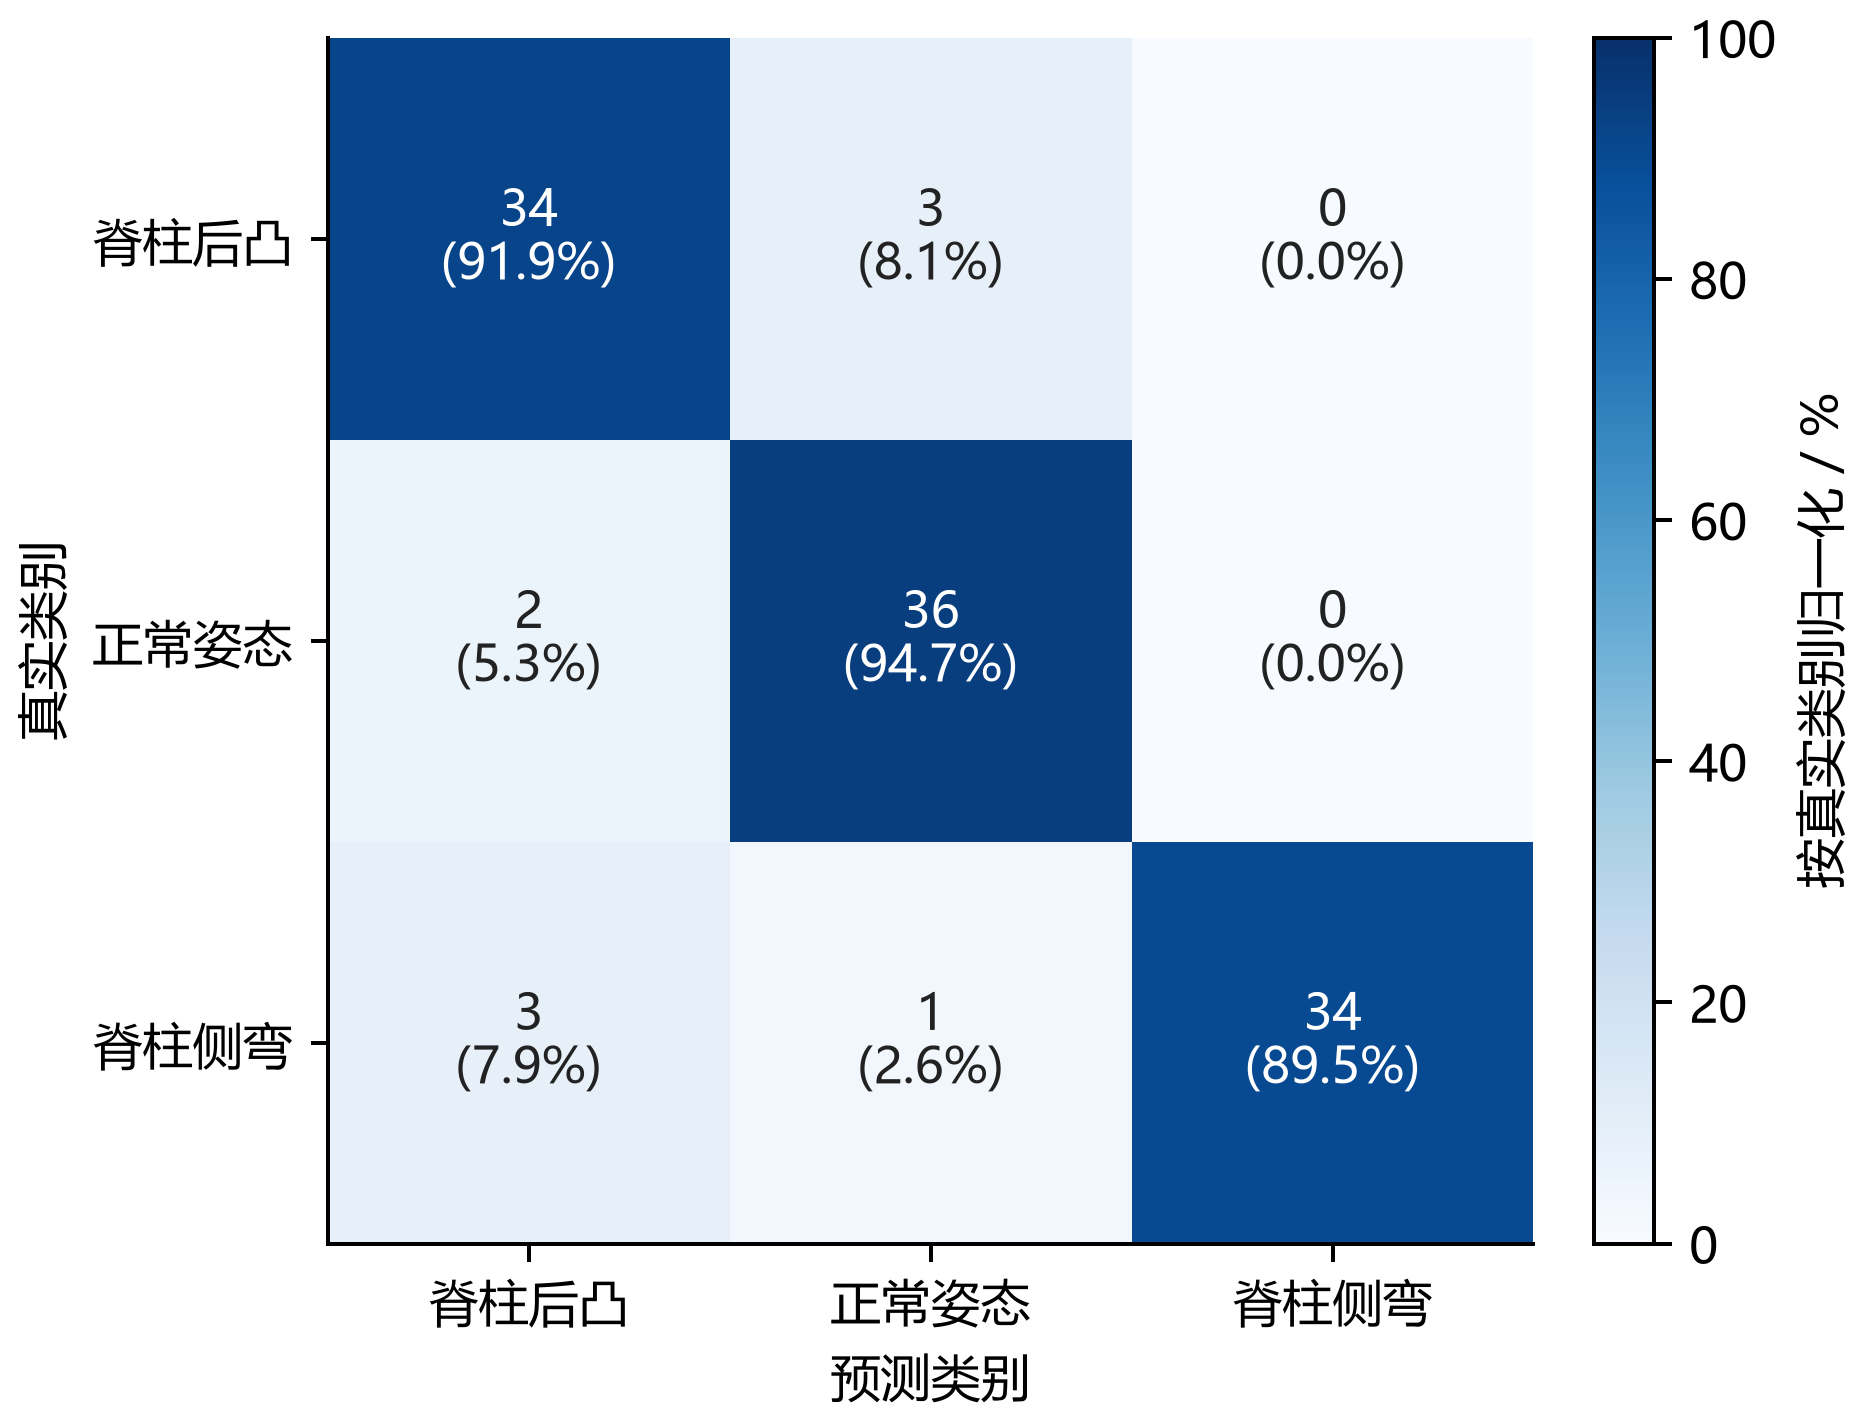
\includegraphics[width=0.72\textwidth]{figures/extratrees_confusion_matrix.png}
\caption{ExtraTrees 模型在测试集上的混淆矩阵}
\label{fig:extratrees_confusion_matrix}
\end{figure}

从混淆矩阵可见，模型对 \texttt{normal} 类别的召回率最高，在 38 个正常姿态测试文件中正确识别 36 个；对 \texttt{scoliosis} 类别的精确率达到 100.00\%，说明测试集中没有其他类别被误判为脊柱侧弯相关姿态；\texttt{kyphosis} 与另外两类之间存在少量混淆，主要表现为 3 个 \texttt{kyphosis} 文件被预测为 \texttt{normal}，以及 3 个 \texttt{scoliosis} 文件被预测为 \texttt{kyphosis}。

\section{结果分析}
实验结果表明，相位比统计特征能够较好地捕捉不同脊柱姿态对 WiFi 信道造成的差异。文件级聚合将多个窗口中的局部时间变化转化为稳定统计量，使模型能够利用完整采集文件中的整体特征进行判断。相比窗口级 TCN，ExtraTrees 在当前数据规模下具有更好的稳定性和测试集表现。

ExtraTrees 的优势主要体现在三个方面。第一，树集成模型适合处理高维统计特征，不需要像神经网络一样从有限样本中重新学习大量时序表示参数。第二，ExtraTrees 的随机特征选择和随机切分阈值能够降低树之间的相关性，提高集成模型的泛化能力。第三，模型训练和推理成本较低，便于在普通 CPU 环境中完成训练、复测和部署。

当前测试结果对应文件级留出测试条件，5 位受试者均出现在训练集、验证集和测试集中。因此，该结果反映的是已登记受试者在相近采集环境下的三类姿态识别能力。后续若面向完全陌生受试者部署，可进一步扩大受试者数量，并采用按受试者分组的划分方式评估跨人泛化能力。

\section{误差模式与结果解释}
从逐类结果看，三类姿态并未表现出完全相同的错误模式。某一类别具有较高精确率，表示模型较少将其他类别误判为该类别；具有较高召回率，则表示该类别的大部分真实样本能够被识别。精确率和召回率所回答的问题不同，因此不能仅根据其中一个指标判断类别识别是否可靠。

混淆矩阵中出现的错误可能来自多种因素。一方面，不同姿态的无线信道分布可能存在重叠，尤其当躯干形态差异较小或受试者保持姿态不稳定时；另一方面，人员体型、相对位置、轻微运动和环境多径也可能改变特征。仅凭混淆矩阵无法确定单个错误的物理原因，若要建立更强解释，需要结合原始信号质量、采集记录和重复实验进行分析。

模型在当前测试集上的结果说明所选特征与分类器在给定条件下具有可行性，但单次文件级随机划分不能估计跨人员性能，也不能充分量化随机划分带来的波动。更完整的评价应包括多次重复划分、置信区间、按受试者分组验证和跨环境测试。由于这些结果尚未在本文当前实验中获得，本文不对其性能作推断，而将其作为后续验证方向。

\section{有效性威胁}
内部有效性主要受到数据划分、参数选择和采集一致性的影响。本文通过文件级划分降低重叠窗口泄漏风险，并隔离测试集；但单次固定划分仍可能受到样本组合偶然性的影响。若采集顺序与姿态标签存在固定对应关系，模型还可能学习时间、设备状态或环境变化等非目标因素。因此，后续实验应随机化采集顺序，并通过重复划分或交叉验证检查结果稳定性。

外部有效性主要涉及受试者、环境和设备覆盖范围。当前评价中不同数据子集包含相同受试者，实验结论主要适用于已覆盖人员和相近采集条件。人员体型、衣着、朝向、收发位置、室内布局和无线设备差异均可能改变信道分布。若目标是面向陌生人员或新环境使用，需要通过分组验证和跨域数据验证模型的泛化能力。

构念有效性关注实验标签与研究概念之间的对应关系。本文分类标签表示预先定义的姿态状态，CSI 模型学习的是这些状态对应的无线信道模式，而不是直接测量脊柱曲率或解剖结构。因此，准确率和 F1 值只能用于评价姿态分类任务，不能转换为医学诊断准确率。实际健康应用仍需要专业人员和标准医学检查建立独立的临床有效性证据。

\section{本章小结}
本章按照研究问题、数据划分、评价指标、模型比较和误差解释组织实验。结果表明，文件级相位比统计特征与 ExtraTrees 的组合在当前留出测试条件下取得了较好的分类性能。与此同时，实验结论受到单次划分、已登记受试者和相近采集环境的限制。通过明确实验协议和有效性威胁，可以将当前结果解释为方法可行性证据，而不是对跨人员或临床性能的直接证明。


% !TEX TS-program = XeLaTeX
% !TEX encoding = UTF-8 Unicode

\chapter{系统实现与检测流程}
\label{chap:implementation}
\defaultfont

\section{系统模块划分}
基于 WiFi CSI 的脊柱姿态检测系统由数据读取模块、特征处理模块、文件级特征构建模块、模型训练模块和检测输出模块组成。各模块按照数据流顺序连接，形成从 CSI 原始数据到脊柱姿态类别输出的完整处理流程。

数据读取模块负责解析 CSI 原始文件，提取时间帧、子载波、接收天线和发射天线信息；特征处理模块负责计算接收天线相位比并进行时间相位展开；文件级特征构建模块通过滑动窗口和统计聚合生成 1620 维特征向量；模型训练模块使用带标签文件训练 ExtraTrees 分类器；检测输出模块根据训练完成的模型输出最终姿态类别。

\section{系统功能设计}
系统采用分层方式组织数据处理与分类功能。数据层负责读取原始 CSI 并形成统一的复数矩阵表示；特征层完成接收天线相位比计算、时间相位展开、窗口组织和文件级统计聚合；模型层负责 ExtraTrees 分类器的训练、保存与加载；应用层接收待检测样本并输出姿态类别。各层之间通过固定维度的数据表示连接，使训练阶段和检测阶段能够复用同一套特征处理流程。

这种功能划分将 CSI 解析、特征变换和分类决策相互分离。一方面，单个处理环节可以独立验证，便于定位数据解析或特征维度错误；另一方面，当采集设备或分类模型发生变化时，可以在保持其他环节不变的情况下替换对应模块，从而提高系统的可维护性和扩展性。

\section{训练流程}
训练阶段首先读取带标签的 CSI 文件，并按照固定随机种子在文件级划分训练集、验证集和测试集。随后，系统对每个文件执行 CSI 解析、接收天线相位比计算、相位展开、滑动窗口生成和文件级统计特征聚合，得到用于分类的 1620 维特征向量。

在模型训练阶段，ExtraTrees 分类器使用训练集文件特征学习分类规则，并通过验证集比较不同配置的表现。最终模型使用 700 棵极端随机树、类别平衡权重、平方根特征采样和固定随机种子。训练完成后，系统保存模型文件和实验指标，便于后续复测和部署。

训练完成后，系统保存分类模型，并记录数据划分、训练配置和评价指标。模型参数与实验元数据分别保存，使后续复测能够恢复与训练阶段一致的数据处理配置，同时避免测试集信息参与模型选择。

\section{检测流程}
检测阶段对新的 CSI 文件执行与训练阶段一致的数据处理流程。系统首先解析复数 CSI，然后以第 0 根接收天线为参考计算相位比，并沿时间维度展开相位；之后生成长度为 512、步长为 256 的滑动窗口，并将该文件的全部窗口聚合为 1620 维统计特征；最后加载序列化后的 ExtraTrees 模型，输出三类姿态之一。

检测流程可表示为
\begin{equation}
X_{\mathrm{raw}}\rightarrow X_{\mathrm{csi}}\rightarrow X_{\mathrm{ratio}}\rightarrow X_{\mathrm{stat}}\rightarrow \hat{y}.
\end{equation}
其中 $X_{\mathrm{ratio}}$ 表示相位比序列，$X_{\mathrm{stat}}$ 表示文件级统计特征，$\hat{y}$ 表示最终检测类别。

\section{复现性验证}
模型训练完成后，本文在独立运行环境中重新加载所保存的模型，并按照训练时记录的数据划分和特征配置对测试集进行复测。复测得到 92.04\% 的测试准确率和 92.08\% 的宏平均 F1 值，分类报告与混淆矩阵均与原始实验结果一致。这表明模型序列化过程未改变分类行为，训练与检测阶段的数据处理流程也保持一致。

\section{应用特点}
该系统不依赖摄像头图像和可穿戴设备，能够在室内 WiFi 环境下进行非接触式姿态感知。系统通过 CSI 相位比特征捕获人体姿态对无线信道的影响，并利用文件级统计特征和 ExtraTrees 集成分类器完成三类姿态检测，具有隐私友好、部署成本低和计算开销较小等特点。


% !TEX TS-program = XeLaTeX
% !TEX encoding = UTF-8 Unicode

\chapter{讨论与适用性分析}
\label{chap:discussion}
\defaultfont

\section{方法结果的含义}
本文实验说明，在当前受试者和采集条件下，接收天线相位比与文件级统计特征能够形成具有类别区分能力的表示。该结果支持“人体姿态差异能够通过无线信道统计模式间接感知”这一研究思路，也说明在样本规模有限时，经过领域知识约束的统计表示可以与树集成模型形成有效组合。

然而，分类性能并不能单独证明模型学习到了唯一且稳定的姿态机理。无线信号同时受到人员、环境、设备和采集过程影响，模型可能利用多个相关因素完成分类。特征重要性能够反映模型内部使用哪些变量进行节点划分，但不等同于物理因果关系。要进一步解释信号变化与姿态之间的联系，需要通过控制变量实验、消融实验和跨条件重复测量排除其他可能因素。

\section{文件级统计表示的优势与局限}
文件级统计表示将长度可变的连续序列压缩为固定长度向量，能够降低单个异常帧和短时扰动对最终判断的影响。均值、分位数和标准差描述整体分布，差分统计描述时间变化强度，正弦和余弦统计保留周期变量的方向信息。对于持续时间较长、类别相对稳定的姿态状态，这种表示与研究对象具有较好的一致性。

统计聚合的主要局限是丢失精细时间顺序。两个具有不同变化过程的序列可能产生相近的分布统计量，短暂姿态转换也可能被完整文件的总体分布稀释。因此，该方法更适合离线文件级状态判断，不应在缺少验证的情况下直接用于快速动作分段或实时连续姿态追踪。若研究目标转向动态过程，需要结合时序编码、状态平滑或分段检测方法保留更多时间结构。

\section{人员与环境泛化}
无线信道具有明显的场景依赖性。受试者体型和动作习惯会改变人体反射特征，人与收发设备的距离和朝向会改变主要传播路径，家具移动和人员走动也会改变多径结构。因此，在相同人员和相近环境中取得的结果，不能直接代表陌生人员或新环境中的性能。

跨人员评价可以采用留一受试者验证或分组交叉验证，使测试人员完全不出现在训练阶段。跨环境评价需要在不同房间、收发位置和时间条件下采集独立数据；跨设备评价则需要考虑天线数量、子载波配置和射频链路差异。当输入维度或硬件特性改变时，原有特征定义可能无法直接迁移，需要重新建立链路对应关系或设计设备无关表示。

提高泛化能力可以从数据和方法两个方向开展。数据层面应增加人员、环境和采集时间的覆盖，并随机化姿态采集顺序；方法层面可以研究归一化、稳健特征选择、域适应和不确定性估计。无论采用何种方法，都应通过独立域测试验证，而不能仅根据训练集增强或模型复杂度推断泛化性能。

\section{潜在混杂因素}
姿态标签之外的因素若与类别同步变化，可能形成混杂。例如，不同姿态按照固定顺序采集时，设备温度、人员疲劳或环境变化可能与类别产生相关；不同类别若在不同位置或时间段采集，模型也可能利用位置和时段特征完成分类。混杂因素不会必然导致低准确率，反而可能产生较高但不可迁移的测试结果。

控制混杂需要在采集设计阶段随机化类别顺序、统一姿态持续时间并记录人员位置和环境状态。在分析阶段，可以按照人员、时间或采集批次进行分组评价，检查性能是否依赖某一批数据。对于错误样本，还应回看信号质量和采集记录，判断其是否与异常帧、姿态保持不稳定或环境扰动有关。

\section{辅助感知与医学应用边界}
本文模型的输入是无线信道状态信息，输出是预先定义的姿态类别。该过程没有直接测量脊柱曲率、椎体结构或其他临床指标，因此研究结果应解释为姿态辅助感知，而不是疾病筛查或诊断性能。即使分类标签使用了与脊柱形态相关的名称，模型仍然只是在当前标注体系下识别无线信号模式。

若未来面向健康监测场景，需要将技术有效性与临床有效性分开验证。技术有效性关注系统能否在不同人员和环境下稳定记录并识别姿态；临床有效性则需要专业医学标准、合适的受试者群体和规范的研究设计，验证系统输出是否与具有临床意义的指标相关。在完成这类验证之前，系统界面和论文表述都应避免使用替代诊断、确认疾病或保证健康结果等结论。

\section{隐私、伦理与数据治理}
\enlargethispage{\baselineskip}
无线感知不直接采集人体图像，能够降低面部和室内视觉信息暴露的风险，但 CSI 数据仍可能间接反映人员存在、活动规律和行为状态。因此，隐私保护不能只依据数据是否为图像判断。研究采集应取得知情同意，说明数据用途、保存期限和访问范围，并尽量减少与研究目标无关的身份信息。

模型部署还应考虑输出的可解释性和误判影响。对于健康相关提示，低置信度或输入质量不足时应允许系统拒绝判断，并向使用者说明结果的不确定性。数据访问、模型更新和结果记录需要建立权限与审计机制，避免无线感知数据被用于未经授权的人员监控。

\section{后续验证路线}
后续工作应按照由受控条件到开放条件的顺序推进。首先，可在相同人员和环境下开展不同时间的重复采集，评价结果随时间的稳定性；其次，采用按受试者分组的评价协议验证跨人员泛化；再次，在不同房间、收发位置和设备条件下建立独立测试集，分析环境和硬件变化的影响；最后，在完成离线稳定性验证后，再研究连续数据流中的在线分段、质量控制和结果平滑。

在方法分析方面，可以开展特征消融和参数敏感性实验。通过分别移除分布统计、差分统计和周期统计，可以判断各类特征的相对贡献；通过改变窗口长度、步长和树数量，可以观察模型对关键配置的敏感程度。所有比较应使用相同的数据划分和评价脚本，并报告重复实验的均值、波动或置信区间。只有实际完成这些实验后，才能对特征贡献和参数稳定性作出定量结论。

\section{本章小结}
本章讨论了文件级统计表示的适用条件、人员与环境泛化、潜在混杂因素、医学应用边界以及隐私伦理问题。当前结果能够支持方法在给定条件下的可行性，但不能代替跨人员、跨环境和临床有效性验证。后续研究需要通过分组评价、独立域测试、消融实验和不确定性处理逐步扩大证据范围。

\cleardoublepage

% !TEX TS-program = XeLaTeX
% !TEX encoding = UTF-8 Unicode

\chapter*{\hfill 结　　论 \hfill}
\addcontentsline{toc}{chapter}{结　　论}
\label{conclusion}
\defaultfont

本文围绕基于 WiFi CSI 的脊柱姿态检测问题，研究了一种非接触式三分类识别方法。该方法利用人体姿态变化对无线信道的扰动作用，将脊柱姿态检测建模为正常姿态、脊柱后凸相关姿态和脊柱侧弯相关姿态的分类任务，并通过接收天线相位比、文件级统计特征和 ExtraTrees 集成分类器实现姿态识别。

本文首先分析了 WiFi CSI 在人体姿态感知中的作用，说明 CSI 幅度和相位能够反映无线传播路径变化。针对原始相位容易受到硬件偏移和公共相位误差影响的问题，本文采用接收天线相位比构造相对相位特征，并沿时间维度进行相位展开。随后，本文使用滑动窗口组织连续 CSI 序列，并将每个原始文件聚合为 1620 维统计特征。最终，本文采用 ExtraTrees 分类器学习统计特征与脊柱姿态类别之间的映射关系。

实验使用 750 个 CSI 原始文件，三类姿态各 250 个样本，并在文件级划分训练集、验证集和测试集。最终模型在 113 个测试文件上取得 92.04\% 的准确率和 92.08\% 的宏平均 F1 值。其中，正常姿态 F1 值为 92.31\%，脊柱后凸相关姿态 F1 值为 89.47\%，脊柱侧弯相关姿态 F1 值为 94.44\%。实验结果表明，基于相位比统计特征和 ExtraTrees 的方法能够有效区分三类脊柱姿态。

本文建立了从 CSI 数据读取、特征处理、模型训练到检测输出的完整技术流程，为基于 WiFi 信号的脊柱姿态辅助检测提供了一种可行方案。该方法具有非接触、低侵入和隐私友好的特点，适用于室内场景下的人体姿态感知研究。后续工作可从受试者规模扩展、跨人泛化评估、幅度与相位融合、环境增强和实时检测流程设计等方面继续展开，以进一步提升系统在实际应用中的稳定性和适用范围。

% !TEX TS-program = XeLaTeX
% !TEX encoding = UTF-8 Unicode

\song\wuhao
\linespread{1.25}
\chapter*{\hfill 参~考~文~献 \hfill}
\addcontentsline{toc}{chapter}{参~考~文~献}
\label{reference}

\begin{thebibliography}{99}
\bibitem{halperin2011csi}
Halperin D, Hu W, Sheth A, et al. Tool release: gathering 802.11n traces with channel state information[J]. ACM SIGCOMM Computer Communication Review, 2011, 41(1): 53.

\bibitem{indotrack2017}
Li X, Zhang D, Lv Q, et al. IndoTrack: Device-free indoor human tracking with commodity Wi-Fi[J]. Proceedings of the ACM on Interactive, Mobile, Wearable and Ubiquitous Technologies, 2017, 1(3): 1-22.

\bibitem{signfi2018}
Ma Y, Zhou G, Wang S, et al. SignFi: Sign language recognition using WiFi[J]. Proceedings of the ACM on Interactive, Mobile, Wearable and Ubiquitous Technologies, 2018, 2(1): 1-21.

\bibitem{svm1995}
Cortes C, Vapnik V. Support-vector networks[J]. Machine Learning, 1995, 20(3): 273-297.

\bibitem{randomforest2001}
Breiman L. Random forests[J]. Machine Learning, 2001, 45(1): 5-32.

\bibitem{extratrees2006}
Geurts P, Ernst D, Wehenkel L. Extremely randomized trees[J]. Machine Learning, 2006, 63(1): 3-42.

\bibitem{tcn2018}
Bai S, Kolter J Z, Koltun V. An empirical evaluation of generic convolutional and recurrent networks for sequence modeling[J]. arXiv preprint arXiv:1803.01271, 2018.

\bibitem{csikit2021}
Forbes G. CSIKit: Python CSI processing and visualisation toolkit[EB/OL]. 2021. https://github.com/Gi-z/CSIKit.
\end{thebibliography}


\backmatter

\end{document}
